\setchapterpreamble[u]{\margintoc}
\chapter{Event Sample,(Re)construction and Particle Identification}
\labch{nu_samples}
In the previous chapters, high-energy neutrino interactions within IceCube was discussed, focusing on how the secondary particles generated from these interactions propagate through the ice. From this, one could deduce that different neutrino flavours can create distinct morphological patterns due to the variety of charged particles produced in the interaction processes. As mentioned in Section \ref{sec:morphologies}, these morphological signatures are crucial in identifying the neutrino flavour, although it becomes particularly challenging in the case of tau neutrino-induced double-bang events. Apart from the complexities of reconstruction, another critical aspect is the selection of astrophysical neutrinos from the overwhelming background of atmospheric muons and neutrinos.

In this chapter, the high-energy neutrino sample used for the analysis presented in this thesis will be detailed, along with the reconstruction method used to identify the particles based on the event's morphology. The chapter will begin with a general overview of the simulation chain in IceCube, followed by a brief overview of the SnowStorm simulations used for the analysis. Lastly, the chapter will discuss the influence of the South Pole IceModel on reconstructed Double Cascade events.

\section{Monte Carlo Simulation} 
\label{sec:mc_sim}
The hunt for astrophysical neutrino interactions in the IceCube detector is conducted without access to actual data, a method known as \textbf{blind analysis}. To develop the selection (rejection) criteria for signal (background) events, and their light yield reconstruction, simulated events are used.\sidenote{In some cases, typically during the development phase of the analysis sample, selection cuts are validated on small subset (10\%) of the experimental data, known as \emph{the burn sample}.} By comparing the distribution of an observable quantity between simulated and real data events, conclusions can be drawn about the detected neutrino population. Hence, simulating how IceCube responds to neutrinos and other particles is essential for comprehending the collected data. 

Event simulation in IceCube is based on commonly used Monte Carlo methods. The simulation framework covers all stages, from the generation and propagation of a primary particle to the emission and propagation of Cherenkov light, and finally, the digitized waveforms recorded by all hit DOMs in IceCube. 

\subsection{Icecube simulation chain}
\label{sec:sim_ic}
The IceCube simulation begins with \emph{a particle generator} that simulates a flux of particles hitting the detector. The primary particle can be a neutrino or a cosmic ray particle reaching Earth's atmosphere. Neutrinos may reach the detector directly, while cosmic rays interact with particles in the atmosphere to produce a shower of particles, from which muons and neutrinos can reach the detector by propagating through ice, forming the so-called atmospheric neutrino and atmospheric muon background.
% %\cite{anis_nugen}

\subsubsection*{Particle Generation}
The software that generates neutrinos is called \texttt{NuGen} (Neutrino Generator) and is based on \texttt{ANIS} (All Neutrino Interaction Simulation). To start the simulation, neutrinos of a selected flavour are drawn from a power-law energy spectrum with an equal probability of being a neutrino or antineutrino. Neutrino directions are sampled from an isotropic distribution and aimed to intersect with an imaginary surface centered on the detector. Each neutrino is then propagated in discrete steps through matter encountered on the way to the detector. For each step, a neutrino interacts with a probability\sidenote{a probabilty that gets stored as propagation weight for each stage and enters in total weight calculations as a \emph{total interaction probability}.} of $1 - e^{-\sigma n \Delta x}$ , where $\sigma$ is the total interaction cross-section and $n$ is the density of nucleons at the location in the Earth. The nucleon density is modelled using \emph{the Preliminary Earth Reference Model (PREM)} \sidecite{earthmodel}, which provides the mass density of the Earth as a function of radius. Because the tau has a short lifetime and a large radiation length, it usually transfers a significant portion of its energy to the tau neutrino produced in its decay (see Section~\ref{sec:leptons_inice}). This leads to substantial ddecrease of overall $\nu_{\tau}$ flux at higher energies, a phenomenon known as \emph{tau-regeneration} \sidecite{tau_regeneration}. This so-called earth effect is also taken into account by the \texttt{NuGen} software. \par
After enough steps, neutrinos will reach the imaginary cylinder defining the detection volume where they are forced to interact somewhere between the projected entry and exit points of the cylinder according to a uniform distribution.In the case of a muon resulting from a CC $\nu_\mu$ interaction far outside the surface, the length at which interactions are required to occur is automatically extended backward based on a parameterization of the muon range in ice. When a neutrino interaction is forced, a weight of $p_{\text{int}} = n\sigma L \exp(-n\sigma L_{\text{before}})$ must be assigned, where $L_{\text{before}}$ is the distance before the selected interaction point where an interaction may have occurred, and $L$ is the total length where an interaction may have occurred. This weight is often combined with the propagation weight to give a total interaction probability weight $w_{\text{int}} = p_{\text{prop}} p_{\text{int}}$. The interaction type is then randomly selected according to CC, NC, and GR cross-sections, and secondary particles are generated for further propagation by another program. In IceCube, single atmospheric and astrophysical neutrinos cannot be distinguished on an event-by-event basis. Therefore, the NuGen-generated neutrinos are used for both atmospheric and astrophysical fluxes. Neutrinos will have weights assigned to them according to the expected (or tested) atmospheric and astrophysical fluxes, and these weights can be used to calculate an expected event rate.
 
To generate atmospheric muons and neutrinos, an adapted version of \texttt{CORSIKA} \sidecite{corsika} is used to simulate the production of muons resulting from cosmic ray showers in the Earth's atmosphere. This process begins with a primary particle, typically a nucleus, initiating a cascading shower of particles upon interaction with the atmosphere. Only neutrinos and muons from these showers are capable of reaching the detector. Due to the impracticality of simulating atmospheric neutrino interactions using \texttt{CORSIKA}, only the muons generated in the showers are transmitted to the detector. The software allows for event weighting based on various cosmic ray models. \texttt{CORSIKA} is currently the exclusive software capable of producing muon bundles, which are large numbers of muons originating from the same cosmic ray shower. However, a major limitation of \texttt{CORSIKA} is its computational expense, as it propagates all particles from a cosmic ray shower, most of which are undetectable in a sub-surface detector like IceCube. To address this drawback, \texttt{MUONGUN} \sidecite{jvs_thesis} was developed to simulate single muons more efficiently and economically by generating them directly around the detector volume. In the context of HESE (which will be discussed in Section \ref{sec:HESE}), the primary background arises from single muons, as muon bundles produce a more continuous light deposition, resulting in a higher likelihood of being vetoed upon entering the detector.
\todo{a block diagram of simulation chain here}
Since flux models more complex than a simple power law are often required, \texttt{NuGen} simulations can be re-weighted to match any arbitrary flux. A weight is assigned to each event that reflects the ratio between the desired flux $n_{\mathrm{expected}} = \Phi(E) $ and the generated fluence of neutrinos. The generated fluence can be expressed as,
\begin{equation}
    n_{\mathrm{generated}} = \frac{N(E)}{\Omega A_\perp}
\end{equation}
where $A_\perp$ is the projected area of the detection surface for each neutrino, and $\Omega$ is the solid angle covered by the simulation, typically $4\pi$ for neutrinos coming from the entire sky. $N(E)$ represents the energy distribution of simulated neutrinos, which, for a power-law distribution with $N_0$ events and a power-law index $\gamma$, spanning from energy $E_{\text{min}}$ to $E_{\text{max}}$, is given by:

\begin{equation}
    N(E) = \frac{N_0 E^{-\gamma}} {\int_{E_{\text{min}}}^{E_{\text{max}}} E^{-\gamma} dE}
\end{equation}

Here, $N_0$ refers to the number of neutrino or antineutrino events, and not the total, when separate fluxes for neutrinos and antineutrinos are known. This implies that $N_0$ represents half of the total number of events generated for each neutrino flavor. Finally, accounting for the interaction weight, the total weight assigned to each neutrino (in units of Hz) is:

\begin{equation}
    \begin{split}
        w &= w_{\text{int}} \frac{n_{\mathrm{expected}}}{n_{\mathrm{generated}}}\\
           &= w_{\text{int}} \frac{A_\perp \Omega \Phi(E)}{N(E)}
    \end{split}
\end{equation}

By summing these weights over all simulated events that pass the event selection, the expected event rate for any desired flux model can be calculated.

\subsubsection*{Secondary Charged Particle Propgation}
Once a particle interaction occurs within the detector volume, the next step is to generate and propagate secondary particles through the ice. Depending on their nature, these secondary particles may undergo further interactions within the ice, with some of them producing detectable Cherenkov light in the detector volume (see Section \ref{sec:particle_propagation} for details). Both atmospheric muons from air showers and secondary leptons, such as electrons, muons, and taus from CC neutrino interactions, are propagated through the ice after they are produced. The software used for lepton propagation is called \texttt{PROPOSAL} (Propagator with Optimal Precision and Optimized Speed for All Leptons) \sidecite{proposal} and is based on the previous implementation \texttt{MMC} (Muon Monte Carlo) \sidecite{MMC_paper}. The lepton production is simplified by assuming that the emission angle is aligned with the incident angle of the primary particle, and that it travels at the speed of light, which are both reasonable assumptions above the energy threshold of 100 GeV. The various propagation effects of different particle types and energies, as described in \ref{sec:leptons_inice}, are taken care of by \texttt{PROPOSAL}. In particular, highly energetic muons are simulated to have long tracks that are predominantly characterized by stochastic energy losses. Electromagnetic and hadronic cascades, as described in Section \ref{sec:hadrons_inice}, are simulated by \texttt{CMC} (Cascade Monte Carlo) \sidecite{Voigt}. It generates individual particle showers by randomly sampling energy losses from the energy-dependent shower parametrization and also takes the LPM-effect into account. The shower parametrizations have been determined by fitting the Cherenkov light yield for a full shower simulation using GEANT4 (Geometry And Tracking) \sidecite{shower_profile,cmc}.

\subsubsection*{Photon Propagation}
\begin{marginfigure}
    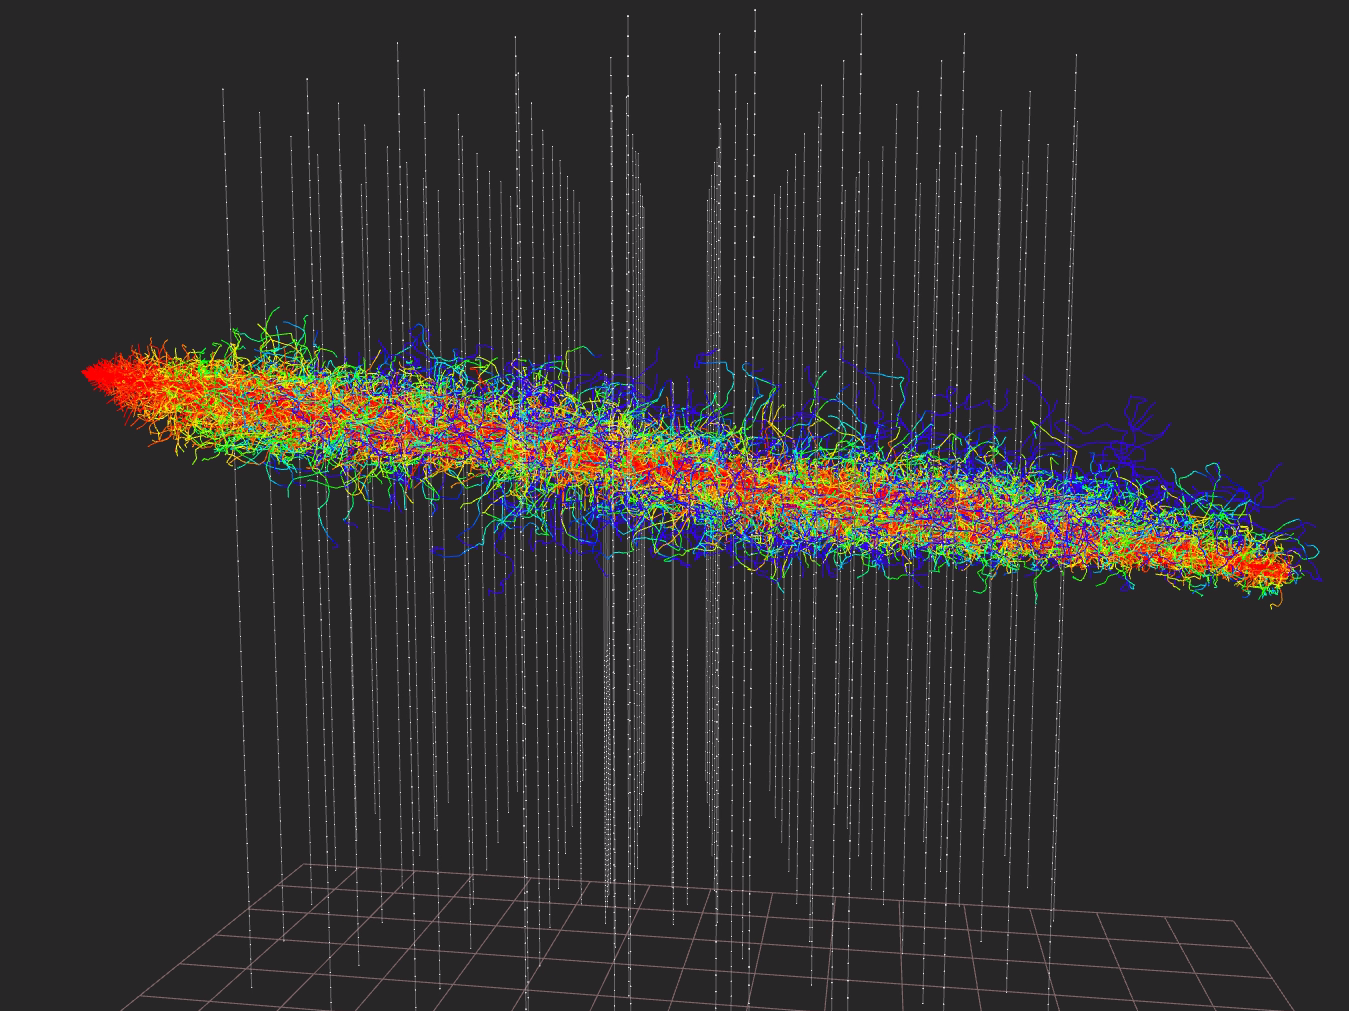
\includegraphics{./figures/EventSample/Icecube_muon_photons.png}
    \caption{Light emission pattern of a simulated muon track event, using the direction propagation program \texttt{CLSim}. The colored lines show individual photon paths through ice, with red indicating earlier and blue indicating later compared to an unscattered photon. Figure taken from \cite{IC_photon_picture}}
    
    \labfig{IC_photons}
\end{marginfigure}
Once all primary and secondary particles have traversed the detector, the next phase of the simulation process involves the emission and propagation of Cherenkov photons from all visible particles or energy losses (as discussed in Section \ref{sec:particle_propagation}). The number of cherenkov photons is proportional to the combined track length of all charged particles, and the refraction index of ice. Individual photon propagation is traced through an \texttt{OpenCL}-based photon-tracking simulation (as shown in \reffig{IC_photons}), known as \texttt{CLSim} \sidecite{clsim}, derived from \emph{Photon Propagation Code} (\texttt{PPC}) \sidecite{PPC_dima}. The SPICE models (as detailed in Section \ref{sec:icemodel})  are used to describe the scattering and absorption of photons. Each photon is tracked through multiple scatterings until it either reaches the collection area of a DOM or, more often, is absorbed. \texttt{CLSIM} harnesses GPUs for photon propagation due to their efficiency in running numerous simple operations (such as photon scattering) in parallel \cite{PPC_dima}. 

Since the direct propagation of photons even by using GPUs can be exteremely time and power consuming, an alternative method is used in IceCube that creates a look-up table that stores the expected timing distribution of photoelectrons at a Digital Optical Module (DOM) for various configurations of the light source and DOM. The concept involves simulating a light source (cascade, track, or flasher) at specific depths and directions multiple times, while tracking the photon yield around the source. Initially, the challenge of creating this table seemed daunting due to the complexity of the problem, as it required a table with 9 dimensions\sidenote{Three for the source position, three for the DOM position, two for the light source orientation, and one for time.}. However, One can take advantage of the approximate horizontal translational and azimuthal symmetry of the ice to reduce the dimensions to 6: depth of the source in ice, zenith angle of the source, displacement vector of the DOM from the source, and time. It is important to note that this approach has its limitations, as it disregards certain effects such as ice layer tilt and anisotropic scattering, which do not adhere to the symmetry assumptions. In recent years, these limitations have been overcome by introducing corrections to scattering lengths (the so-called \emph{effective distance correction}), which was done while developing the double cascade reconstruction \sidecite{marcel_thesis} that will be explained in Section \ref{sec:PID}, and also by introducing corrections directly in modelling of the ice to account for ice anisotropy and tilt corrections, see Section~\ref{sec:icemodel} for details. Initially, \texttt{Photonics} was used to predict and store the expected photon flux in a multi-dimensional histogram structure, but this method had drawbacks such as binning issues and inaccuracies at great distances. Currently, a more effective approach involves fitting the photoelectron distribution obtained from \texttt{CLSim} or \texttt{PPC} to a tensor product B-spline surface \sidecite{splines}. This offers the advantage of having a smooth function of all 6 coordinates and can address unphysical fluctuations caused by limited statistics through the use of regularization.

\subsubsection*{Detector Simulation}
The detector's response is the final step in the simulation process. The PMT's sensitivity depends on the wavelength and angle of the incoming photon, as well as its quantum efficiency. This means that not every photon will trigger the PMT. The simulation takes into account the varying PMT sensitivity for each photon. Additionally, the simulation considers the angular acceptance of photons, accounting for local scattering variations in the ice. The PMT hardware has been thoroughly calibrated and studied in the lab \sidecite{PMT_paper}, and these results have been incorporated into the simulation. It's important to model the transit time and jitter of the PMT in the simulation, as these factors affect the timing and width of the pulse. Furthermore, all triggers used in real-time data collection at the South Pole are also included in the simulation. This final step in the simulation process completes the creation of a simulated event.


\subsection{SnowStorm Simulation}
\label{sec:snowstorm}
As described in previous section, specifically for photon propagation stage precise knowledge of ice is important. While we use calibration measurements to estimate the detector properties, this only provides limited precision. When conducting simulations, which are crucial for estimating the detector's response, one need to be careful not to assume specific detector properties. For most of the IceCube analyses so far, variations of the detector response were included using a particular strategy: A set of Monte Carlo simulations with \emph{baseline} values of all systematic parameters was created to estimate event rate in the analysis. The baseline value of a systematic parameter is its most likely value determined from calibration. Variations of this baseline event rate caused by a different, \emph{off-baseline}, detector response were estimated using different \emph{discrete systematics sets}. The combination of discrete baseline and systematics sets allows the estimation of the analysis variables as well as their variation with the detector systematics. This variation is typically assumed to be small and estimated with a low-order Taylor expansion. The off-baseline systematics sets are then used to estimate the coefficients of this expansion.
\begin{marginfigure}
    \vspace*{-7.5cm}
	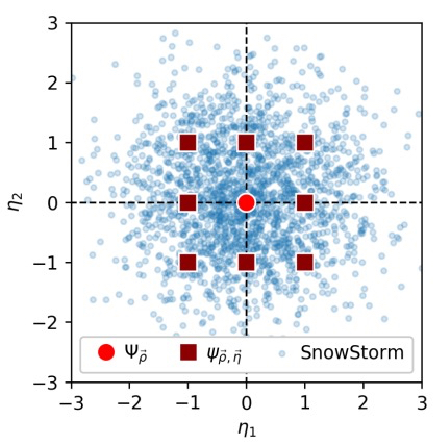
\includegraphics{./figures/EventSample/snowstorm.pdf}
	\caption{Illustration of the SnowStorm method described in the text. It depicts the contrast between numerous discrete shifts in nuisance parameters (indicated by red squares), each necessitating an entire Monte Carlo set, in comparison to a single SnowStorm Monte Carlo (represented by small blue dots). Figure taken from \cite{snowstorm}}
	\labfig{snowstorm}
\end{marginfigure} 
A new approach to model detector systematic uncertainties has been developed in IceCube called, \textbf{SnowStorm Method} \sidecite{snowstorm}. The significant difference compared to the discrete systematics approach described above is that each detector systematic parameter continuously varied while generating the MC events, as visualized in \reffig{snowstorm}. Using the SnowStorm method, one obtains a single MC set representing all variations in the detector response. This can help an analysis by reducing the bookkeeping effort necessary for using multiple discrete sets, studying variations in a large number of detector systematic parameters at once without loss in statistics, and allowing analyses of different event selections to use the same MC set and "marginalize" over all detector systematic parameters that are not relevant for a single analysis.

The analysis presented in this thesis uses simulations generated using this aforementioned novel method. It involves uniform and independent sampling distributions for all relevant parameter uncertainties in the flavor analysis. These simulations cover all three flavors of neutrinos and were created using the SPICE-3.2.1 icemodel. They were designed for general use and were also utilized by several other IceCube analyses simultaneously, see \sidecite{erik_thesis} and \sidecite{richard_thesis} for details. The simulation sets were developed for primary neutrinos in the energy range of $E_{\nu} = $[100 GeV - 1 PeV] assuming a single power law of $E_{\nu}^{-1.5}$, and in the range [1-100 PeV] with a $E_{\nu}^{-1}$ spectrum. The harder spectrum is generally chosen, particularly for higher energy datasets, to ensure a sufficiently large number of events at those energies. Using the weighting method described previously, one can reweight the neutrino events to match any desired spectrum.

\begin{marginfigure}
	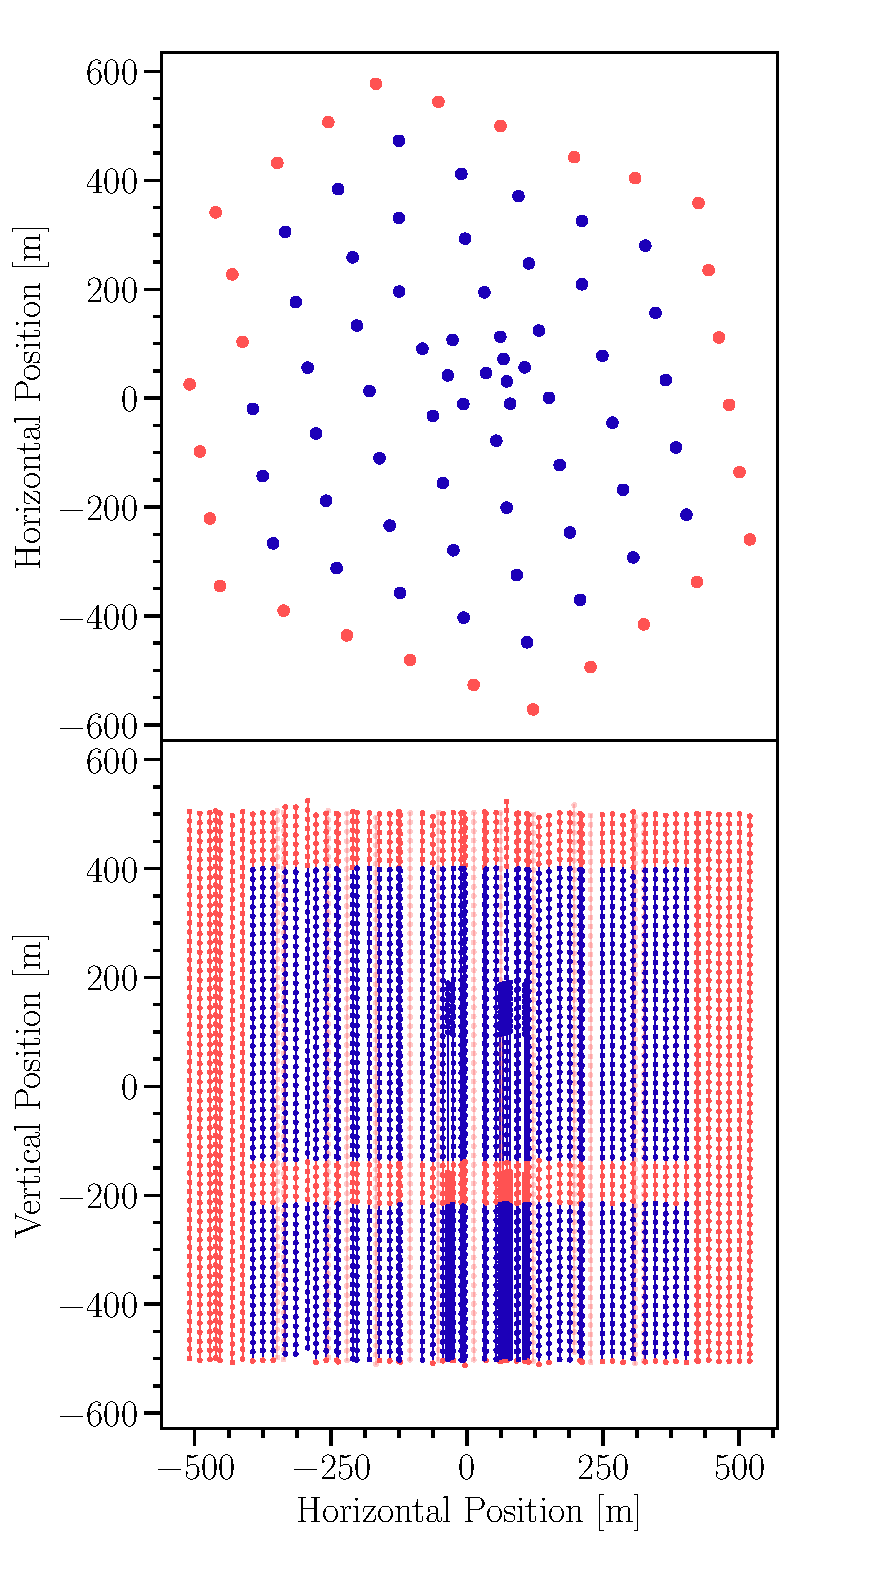
\includegraphics{./figures/EventSample/veto_diagram_vertical.pdf}
	\caption{The top view (above) and side view (below) display the veto DOMs and the DOMs within the fiducial volume for HESE. DOMs highlighted in red represent the veto region, while those in blue define the fiducial volume. Events where the initial detected light comes from the veto region are excluded from the analysis. Figure taken from \cite{HESE7_sample}.}
	\labfig{veto_region}
\end{marginfigure}
\section{High Energy Starting Event (HESE) sample} 
\label{sec:HESE}
The High Energy Starting Events (HESE) selection is a comprehensive, all-sky, all-flavor sample of astrophysical and atmospheric neutrinos observed in IceCube. This selection process led to IceCube's first significant milestone: the discovery of an astrophysical neutrino flux \sidecite{Evidence_paper}. Subsequently, a particle identifier was developed using this sample with added years of data, eventually finding two tau neutrino candidates in IceCube \sidecite{HESE7_sample,Juliana_paper}. For the analysis presented in this thesis, this sample was again used, along with some updates in Self-Veto calculations, that shall be introduced in Section~\ref{sec:selfveto}. The concept behind HESE is to establish a veto region on the detector's outer edges to select only events where the initial Cherenkov photons are detected inside the fiducial volume. As shown in \reffig{veto_region}, the veto region includes the outer strings, a top layer of 90 m, a central layer of 80 m around the dust layer, and a 10 m bottom layer. The very thicker veto at the top is essential for filtering out atmospheric muons entering from above. However, the veto can be thinner at the bottom of the detector since up-going atmospheric muons do not exist. The inclusion of a veto around the dust layer is crucial, as horizontal events passing through this highly absorptive region can mimic starting events. To pass the veto, events must deposit fewer than 3 photoelectron (PE) in the veto region out of the first 250 PE recorded within the fiducial volume, and a minimum total charge of 6000 PE is required to ensure high-energy events are selected.

The HESE selection is particularly powerful due to its simplicity, as it does not rely on complex reconstructions, making it robust against changes in filtering or reconstruction algorithms. The fact that it is an all-flavour sample, can help break degeneracies caused by different neutrino flavors producing similar event patterns. Additionally, the all-sky nature of HESE allows for the study of the zenith distribution of events, which can distinguish between atmospheric and astrophysical neutrinos. However, HESE does have limitations: the high-energy threshold introduces uncertainty in estimating background contributions and astrophysical parameters, and the veto region reduces the detector's effective volume. An extension of HESE to lower energies, known as Medium Energy Starting Events (MESE), has been developed \sidecite{Jvs_MESE} (and recently updated \sidecite{MESE_ICRC}) to overcome some of these limitations.

\begin{marginfigure}
	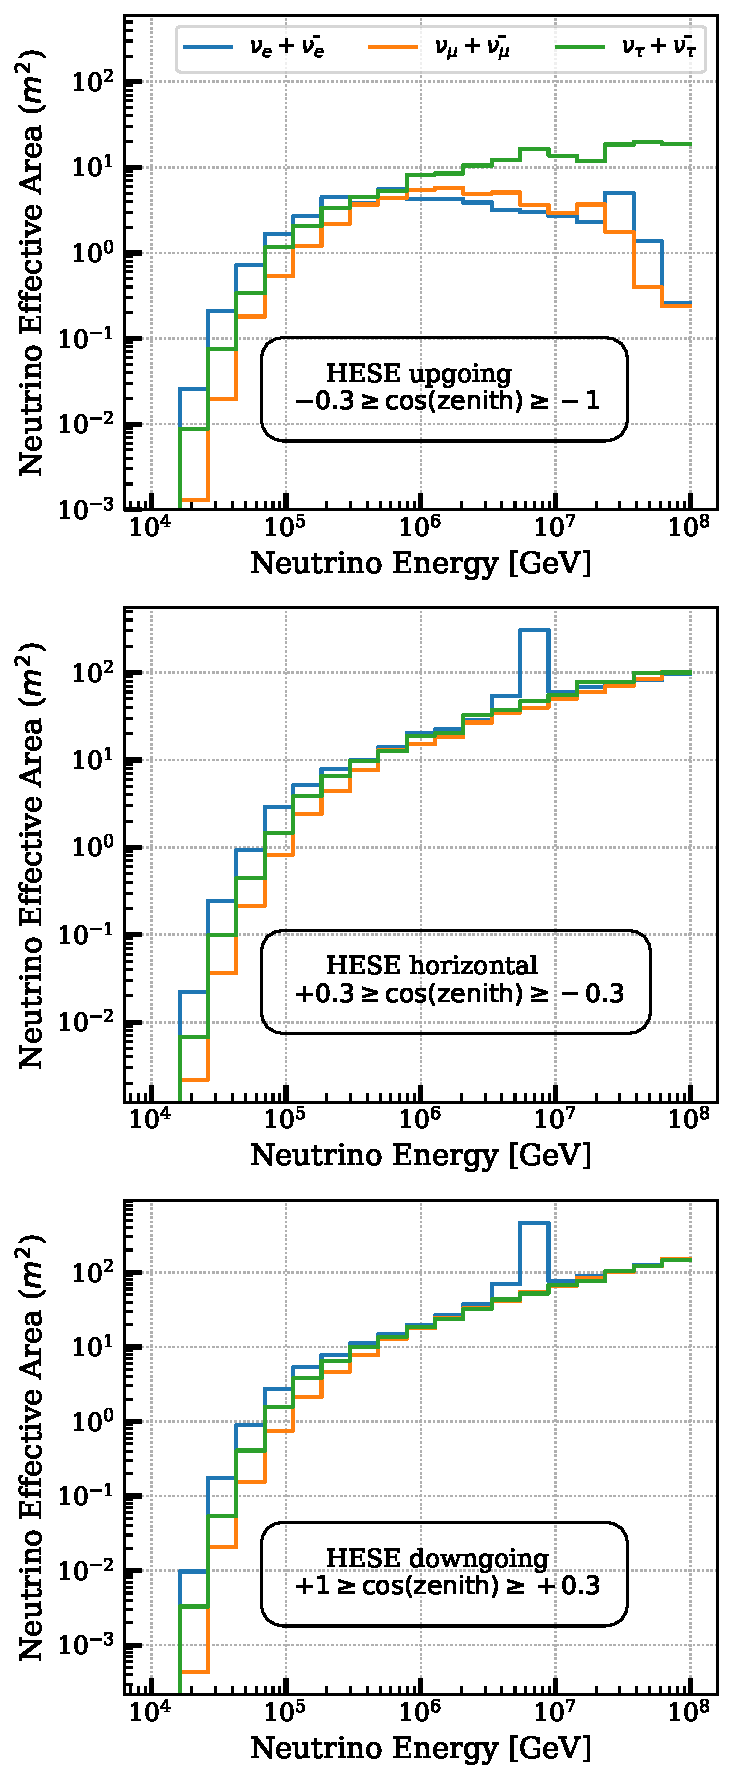
\includegraphics{./figures/EventSample/HESE_Eff_area.pdf}
	\caption{The neutrino effective areas for the high-energy starting event selection as a function of neutrino energy. The distributions are shown for all neutrino flavors, broken down by various zenith angle ranges.}
	\labfig{eff_area}
\end{marginfigure}

Despite of rejecting a significant fraction of atmospheric background, HESE retains the majority of astrophysical neutrinos within its fiducial volume. The neutrino effective area of the HESE sample, increases with neutrino energy due to the larger amount of visible light deposited (see \reffig{eff_area}). At energies above a few hundred TeV, the effective areas become similar across all flavors, except the Glashow resonance of $\bar{\nu_e}$ at 6.3 PeV. However, at lower energies, the effective area varies by flavor due to differences in energy deposition during charged-current interactions, with electron neutrino interactions producing the highest effective area due to the nearly complete energy deposition in electromagnetic and hadronic cascades. For different zenith angles, the effective area decreases as the zenith angle increases, particularly in the up-going region at high energies. This is a result of Earth absorption, which becomes significant for neutrinos above approximately 1 PeV. The distinction between tau neutrinos and other flavors at the highest energies is due to the phenomenon of tau regeneration, where the tau neutrino regenerates after the decay of a tau lepton. Muon neutrino interactions, on the other hand, produce muons that deposit only part of their energy before escaping the detector, resulting in a higher detection threshold. Neutrino interactions, especially for $\nu_\tau$, exhibit effective areas between those of $\nu_\mu$ and $\nu_e$.

\subsection*{Atmospheric Neutrino Self-Veto}
\label{sec:selfveto}
As mentioned in Section~\ref{sec:atm_nu}, high-energy cosmic ray showers produce many neutrinos and muons, which are the only particles able to reach underground detectors such as IceCube. When atmospheric neutrinos reach the detector, they are typically accompanied by other particles from the same CR shower, mostly muons. The chance of a detectable muon accompanied with an atmospheric neutrino is called \textbf{the atmospheric self-veto probability}. Several things affect this probability, such as the type, energy, and direction of the neutrino. In the case of high-energy CR showers, some muons may reach the detector and \emph{trigger} the veto that marks the event as background. The likelihood of rejecting an atmospheric neutrino through this self-veto mechanism increases with higher neutrino energy and more vertical shower angles. With such a modelling, one effectively suppresses the flux of atmospheric neutrinos, in down-going region\sidenote{This process only applies to downward-moving atmospheric neutrinos because muons cannot reach IceCube from below the Earth}. \textbf{The passing fraction} of atmospheric neutrinos—defined as the fraction that is not accompanied by a detectable muon from the same CR shower—varies with both neutrino energy and zenith angle \sidecite{pass_frac}. It tends to increase at larger zenith angles, as muons must travel farther through the atmosphere to reach IceCube, as shown in \reffig{passing_frac1}. At neutrino energies greater than 100 TeV, the contribution from astrophysical neutrinos begins to outweigh the atmospheric background, improving IceCube's ability to detect astrophysical neutrinos as indicate din \reffig{passing_frac2}.

\begin{marginfigure}
	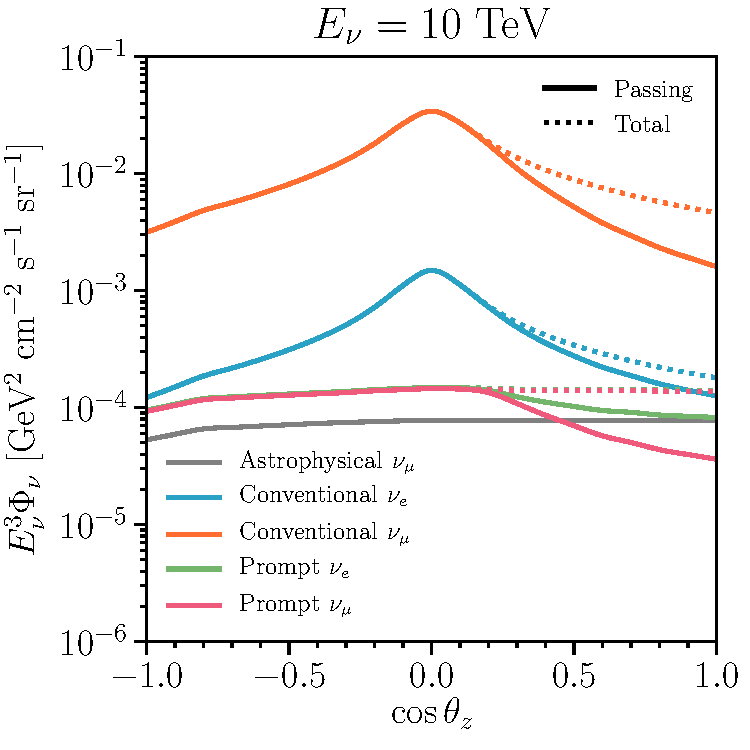
\includegraphics{./figures/EventSample/fig1_fluxes_10.pdf}
	\caption{The Atmospheric neutrino fluxes at \( E_\nu = 10 \, \text{TeV} \). The plot shows the fraction of the flux that is \textbf{not} vetoed, known as \textbf{passing fluxes} (solid lines), alongside the total flux entering the detector (dashed lines) as a function of the cosine of the zenith angle. Figure is adapted from \cite{pass_frac}.}
	\labfig{passing_frac1}
\end{marginfigure}
The passing fractions used in the analysis presneted in this thesis is based on the calculations derived in \sidecite{pass_frac} a formalism used in 7.5 years of HESE analysis \cite{HESE7_sample} through the \texttt{nuVeto} package \sidecite{nuveto}. The previously used calculations are further updated using MCEq package, MCEQ, a tool designed to solve the cascade equations governing cosmic ray-induced showers, allowing for more precise and computationally efficient predictions of atmospheric lepton fluxes \sidecite{MCEq}. 
\begin{marginfigure}
	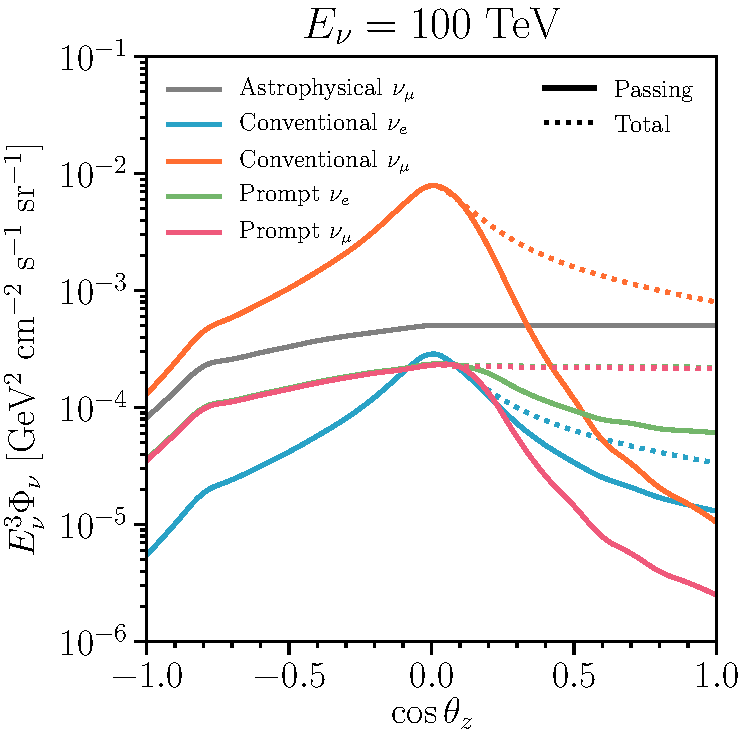
\includegraphics{./figures/EventSample/fig1_fluxes_100.pdf}
	\caption{The atmospheric neutrino fluxes and the effect of self-vetoing are displayed for a neutrino energy level of \( E_\nu = 100 \, \text{TeV} \), see caption of \reffig{passing_frac1}. Figure atken from \cite{pass_frac}.}
	\labfig{passing_frac2}
\end{marginfigure}

\section{Maximum Likelihood Event Reconstruction}
\label{sec:reco}
With the aforementioned HESE sample, next step is to infer the properties of these events—primarily energy, direction, and the deposited light pattern (morphology). To do so, it is necessary to \emph{reconstruct} each individual event. The reconstructed properties are then used to create probability density functions (PDFs) that facilitate likelihood fits for making the desired physics measurements (as outlined in Section~\ref{sec:analysis}). Therefore, it is crucial to reconstruct the event properties as accurately as possible. The analysis presented here utilizes a maximum-likelihood estimation (MLE) approach, called \texttt{millipede} for event reconstruction. 

\texttt{millipede} aims to maximize the likelihood of the observed light pattern from an event, given a specific source hypothesis. The input data comprises individual pulses detected by Digital Optical Modules (DOMs), expressed in terms of charge (measured in photoelectrons (PEs)) and time. These pulses are deconvolved from the digitized waveforms using established single-photoelectron (\texttt{SPE}) pulse templates. The likelihood function compares the observed data to the expected data for a given hypothesis and adjusts the parameters to maximize this likelihood, details of which can be found in \sidecite{energy_reco}.

The expected number of photons detected at DOM $j$ follows a Poisson distribution characterized by a mean $\lambda_j = \Lambda_j E$, where $\Lambda_j$ represents the expected photon yield from a 1 GeV cascade at DOM $j$, and $E$ signifies the cascade's energy, stored in tabulated form as photo splines \sidecite{splines}, which were originally developed and used in an analysis similar to one presented in this thesis \sidecite{marcel_thesis} and now have been updated with newer icemodel\sidenote{to account ice layer tilt and anisotropy due to birefringence (see Section~\ref{sec:icemodel} for details) separately} \sidecite{updated_recotables_tianlu} \footnote{These updated tables are used in the analysis presented in this thesis}. The likelihood of detecting $k_j$ photons at DOM $j$ for a cascade with energy $E$ is given by:

\begin{equation}
    L_j = \frac{(E \Lambda_j)^{k_j} e^{-E \Lambda_j}}{k_j!}
\end{equation}

By taking the logarithm and summing over all DOMs, including noise hits $\rho_j$, along with an expansion to include multiple light sources $i$ and timing information, the log-likelihood can be expressed as:

\begin{equation}\label{eq:millipede_llh}
    \ln L = \sum_{i,j,t} \left( k_{jt} \ln(E_i \Lambda_{ijt} + \rho_{jt}) - (E_i \Lambda_{ijt} + \rho_{jt}) - \ln(k_{jt}!) \right)
\end{equation}

The hypothesis to be compared encompasses the event parameters $(x_s, y_s, z_s, t_s, \theta_s, \phi_s, E_s)$, which define the source's location, time, direction, and energy respectively. 

\marginnote{\begin{kaobox}[title=\textbf{Bright DOM}]
    A Bright DOM generally refers to a situation where a high energy event occurs close to a string, and in first pulse itself, a large amount of charge is observed. Emperically, this \emph{large amount of charge} is assumed to be 10 times the average observed charge of the event.
\end{kaobox}}

\marginnote{\begin{kaobox}[title=\textbf{Saturated DOM}]
    A DOM is considered saturated if its PMT reaches saturation. This can happen if an event occurs close to a string or a very high energy interaction occurs, producing many photons that gets collected by the PMT. These DOMs generally don't have a \emph{complete} digitized waveforms, making them unsuitable to be used in likelihood based reconstruction.
\end{kaobox}}
\texttt{millipede} offers a comprehensive set of configurations that allow users to define how photons are organized in terms of time bins, the magnitude of changes in various parameters, and the exclusion of specific modules from the likelihood calculation. One crucial aspect of these settings is the selection of an ice model for data reconstruction. This model plays a vital role in predicting the expected number of photons that will reach a DOM based on variables such as distance and direction from the source. Additionally, the ice model can influence the timing information of these photons \sidecite{BFR_paper}, which is critical for accurate event reconstruction. \sidenote{Different approaches to model the ice at the South Pole can significantly affect the reconstructed properties of an event, in particular the double cascade reconstruction using \texttt{taupede} (see Section~\ref{sec:icemodel_checks} at the end of this chapter for such detailed checks)}. As for exclusions of certain modules, \textbf{bright DOMs} and \textbf{Saturated DOMs} are excluded from the likelihood fit because they may introduce bias by contributing excessively to Equation~\ref{eq:millipede_llh}. These particular DOMs generally account for a significant portion of the total observed charge. Hence, bright and saturated DOMs alongwith other DOMs that may have failed during the Run are generally labelled as \emph{Bad DOMs} and are collectively excluded from the reconstruction 
\marginnote{\begin{kaobox}[title=\textbf{DeepCore DOM exclusion}]
    DeepCore DOMs have traditionally been excluded from high-energy reconstruction methods like \texttt{millipede}  because it uses spline tables that assume a uniform single photoelectron (SPE) template for all DOMs. However, the higher quantum efficiency of DeepCore DOMs results in significantly different charge collection, meaning their SPE templates differ from those of other DOMs. Recent efforts have updated simulations to address this issue (as will be discussed in Section \ref{HESE12}).
\end{kaobox}}. \texttt{millipede} framework helps reconstruct single and double cascades, along with track source hypotheses. Although they all use the same likelihood from Equation~\ref{eq:millipede_llh}, they each have different ways to define sources. The hypothesis that fits the observed data best is found by comparing maximum likelihood values, which gives an idea of the interaction type in the detector.

\textbf{\texttt{monopod}}: \texttt{monopod} does a simple one-particle cascade energy fit, in other words it assumes a single light source. It minimizes parameters such as the cascade's deposited energy, neutrino direction (azimuth and zenith), cascade vertex position $(x, y, z)$, and vertex time, represented as, $\vec{h} = (x, y, z, t, \theta, \phi, E)$ \sidecite{jvs_thesis}. The reconstructed vertex here refers to the shower maximum, which is the peak of the longitudinal energy loss profile and is typically displaced from the interaction vertex by several meters in the considered energy range.

\textbf{\texttt{taupede}}: The double cascade fitting algorithm, \texttt{taupede}, maximizes the likelihood of two energy depositions with energy $E_1$ and $E_2$ respectively, separated by distance $L_{\mathrm{dc}}$. The second cascade's direction matches the first, and its vertex is determined by the first cascade's vertex, direction, and double cascade length $L_{\mathrm{dc}}$. The parameters for the double cascade hypothesis are $\vec{h} = (x_1, y_1, z_1, t_1, \theta, \phi, E_1, L_{\mathrm{dc}}, E_2)$, with the tau traveling in the same direction as the incoming neutrino due to Lorentz boosting. The light yield and timing at each Digital Optical Module (DOM) are compared with expected values from the two energy depositions. For the second cascade's timing, the conditions are $|\vec{x}_2 - \vec{x}_1| = L_{dc}, \quad t_2 - t_1 = c L_{dc}$\sidenote{assuming tau travels through the ice at the speed of light $c$.}. 

\textbf{\texttt{mumillipede}}: Track-like events are parameterized as multiple cascades along its path. The total deposited energy is given by $E_{\text{dep}} = \sum_k E_k$. Although the deposited energy is not a reliable indicator of the primary neutrino energy, the parameters related to direction and time are vital for neutrino point-source searches.

The algorithm outlined above relies on the quality of the seed, which serves as the initial hypothesis $\vec{h_0}$. This seed is adjusted until a satisfactory match is achieved between the expected and actual light yield. This process has proven challenging, especially in the case of \texttt{taupede}, where the seed combines aspects of both a cascade and a track. Locating an appropriate seed is difficult, and the reconstruction process is influenced by the choice of seed. To reduce this influence, one can either modify the seed or increase the number of iterations\sidenote{All algorithms are run multiple times, starting with a provided \texttt{seed}, where each subsequent iteration uses the output from the previous one, as explained in Section~\ref{sec:PID}.}; however, both approaches result in greater computational expenses. To tackle the challenges associated with reconstructing double cascade events, an improved method for implementing the \texttt{taupede} fit was developed \sidecite{marcel_thesis}. This method effectively converts the fitting process into a \emph{brute-force} approach, where multiple hypotheses are explored and evaluated.

Simple reconstruction methods like \textbf{\texttt{LineFit}} and \textbf{\texttt{SPEFit}} provide fast initial estimates for event properties. These methods use limited event information, such as the first photon arrival time or total photoelectrons, without relying on detailed ice properties. The results are then used as seeds for more refined algorithms like \texttt{millipede}. For cascade-like events, simpler MLE methods are used to find a charge-weighted mean position of the source, providing an efficient first estimate.


\section{Particle Identification of High Energy Neutrinos}
\label{sec:PID}
Event reconstruction is performed using the aforementioned \texttt{millipede} framework, which enables the identification of different interaction types by assigning \textbf{a particle identifier (PID)} to each reconstructed event. The PID provides the probability that an event corresponds to a particular type of interaction. \textbf{A ternary topology identifier} has been developed (initially developed in \cite{marcel_thesis} and later used to find first two tau candidates in IceCube \sidecite{Juliana_paper}) based on the three event topologies—single cascade, double cascade, and track. By using these IDs, Monte Carlo templates are constructed to extract the contribution fractions from each neutrino flavor (see \refch{analysis}).

The analysis presented in this thesis has two main goals: to identify double cascades produced by tau neutrinos and to determine the flavor composition of astrophysical neutrinos. Given the complexity of detecting double cascades and the susceptibility of the reconstruction algorithm to failures and dependence on the initial seed hypothesis, the classification process uses a combination of algorithms offered by the \texttt{milllipede} framework, which run in parallel on each of the HESE events that provides likelihood for the three event morphologies. 

As mentioned before, these methods are \texttt{seed} dependent, hence to start with, all selected HESE events are reconstructed using first-guess algorithms to determine their vertex and direction. Result of these quick methods provides an initial fit for the event's position and trajectory, serving as a seed for \texttt{monopod}, which performs a fit with four iterations.

Generating a reliable seed for \texttt{taupede} is more complex. Multiple seeds are constructed using the monopod fit and generated with varying lengths (10, 25, 50, and 100 meters), each shifted forward, backward, or centered along the direction of the seed in bruce-force way \sidecite{marcel_thesis}. An amplitude-only \texttt{taupede} fit is performed for each of the 12 seeds \sidenote{4 length seeds shifted 3 times, giving total of 12 seeds}, and the three best-performing seeds are selected for a full fit, performing 4 iterations of fits again, which incorporates photon arrival times at the Digital Optical Modules (DOMs). This method accounts for the diverse photon arrival patterns produced by scattered photons in single energy depositions \sidecite{Juliana_thesis}.
\marginnote{\begin{kaobox}[title=\textbf{Quality Criteria for \texttt{taupede} fit}]
    The final-best fit of \texttt{taupede} is accepted only if all the following criteria are satisfied:\\
    \texttt{taupede} Fit is converged\\
    Energies of both of the fitted cascades $E_1,E_2 \geq 1 \, \text{TeV}$\\
    Both cascades are \emph{softly} contained (vertex $\leq 50 \, \text{m}$ outside detector)\\
    Opening angle between \texttt{taupede} and \texttt{mumillipede} fit $\leq 30^\circ$
\end{kaobox}}
The tracks are reconstructed using the \texttt{SPEFit} algorithm, which iteratively (16 times) fits a track based on the first photoelectron detected at each DOM. Although the \texttt{mumillipede} algorithm could also reconstruct tracks, it is computationally intensive, so \texttt{SPEFit} is preferred. Finally, \texttt{mumillipede} unfolding is performed along the directions determined by each topology fit (\texttt{monopod}, \texttt{taupede}, and \texttt{SPEFit16}), allowing for a comparison of likelihood values for each hypothesis. The best fit is selected for final classification based on the highest likelihood value.

Since identifying tau-induced double cascades is main goal of this process, the comparisons of the three likeelihoods is not the only proxy by which the classifier selects a double cascade event. First, the \texttt{taupede} fit is vetted through \textbf{Quality Criteria}, on the basis of containment, and reconstructed properties. If these criteria are satisfied\sidenote{If any of the quality checks are failed, the event is assigned track or cascade morphology depending on which of the fit's likelihood is higher.}, further classification is performed using additional selection criteria based on observables derived from reconstructed quantities, described below:

\marginnote{\begin{kaobox}[title=\textbf{Direction definitions in IceCube}]
\emph{The zenith angle} ($\theta$) gives the direction of particle origin with respect to the vertical axis that points towards the surface of the ice and upward from the South Pole.\\
A zenith angle of \(0^\circ\) indicates a particle moving directly downward in the detector, \(90^\circ\) corresponds to horizontal propagation, and \(180^\circ\) signifies a particle moving directly upward.\\
\\
\emph{The azimuth angle} ($\phi$) gives the direction of particle origin with respect to the horizontal x-axis of the IceCube coordinate system (see Section~\ref{sec:IC_coordinate})
\end{kaobox}}
\textbf{The reconstructed direction} of a particle is indicated by its zenith and azimuth angles. The azimuthal angle is not useful for distinguishing between atmospheric and diffuse astrophysical neutrino fluxes since both are isotropically distributed. However, it is important for addressing systematic uncertainties in reconstructed track length due to anisotropic light scattering in the ice. However, zenith angle provides a reliable estimate of the neutrino's initial trajectory, espfecially for tracks, which can be reconstructed more accurately than cascades.

\textbf{The total deposited energy ($E_{\text{tot}}$)} refers to the visible energy in the detector, calculated as the sum of all contained energy losses along the best-fit hypothesis. The total deposited energy serves as a lower limit for neutrino energy and is used as a direct observable in the likelihood fit (see Section~\ref{sec:hists}). Not all energy is deposited in the detector; some may be carried away by secondary neutrinos from tau decays or by muons that leave the detector, while some energy may remain invisible during hadronic showers. Therefore, the sensitivity of total deposited energy to primary neutrino energy varies by event morphology. In single and double cascade topologies, the initial energies of electron and tau neutrinos can be constrained more accurately than those of muon neutrinos, as muon usually leaves the detector and also the energy losses are stochastic, making the proxy weaker. 
\begin{marginfigure}
	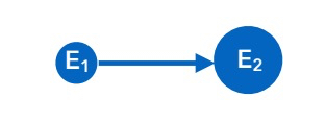
\includegraphics{./figures/EventSample/EA.pdf}
	\caption{A sketch of energy asymmetry, it is a measure of the relative distribution of total deposited energy between the two cascades, as defined in \ref{eq:EA}. Sketch is adapted from \cite{marcel_thesis}.}
	\labfig{EA_fig}
\end{marginfigure}

\textbf{The Reconstructed length ($L_{\mathrm{reco}}$)}, represents the distance between two cascades in double cascade events, is a critical observable for tau-neutrino interactions. 

\textbf{The energy asymmetry ($E_{\text{A}}$)} measures the distribution of deposited energy between the two cascades in a double cascade event. It is defined as,
\begin{equation}\label{eq:EA}
    E_{\mathrm{A}} = \frac{E_1-E_2}{E_1+E_2}
\end{equation}
where $E_1$ and $E_2$ are reconstructed energies of the first and the second cascades. A \emph{true}\footnote{\emph{true} event morphologies are assigned by going through produced charged particles at Secondary Charged Particle Propgation stage of the simulation chain (see Section~\ref{sec:sim_ic}). Looking at the type of particles, their energy depositions and positions within the detcetor volume, a morphology is assigned to the event.} single cascade has an energy asymmetry of 1\sidenote{since there is no second energy deposition technically, $E_2=0$ for a true single cascade}, while a double cascade can have any value between -1 and 1, depending on the kinematics of the neutrino interaction. This variable hence, is an excellent estimator to distinguish between a single and a double cascade.

\begin{marginfigure}
	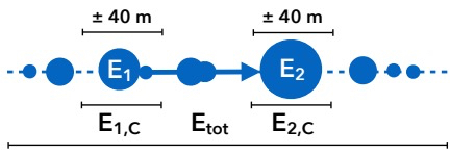
\includegraphics{./figures/EventSample/EC.pdf}
	\caption{A sketch of Energy Confinement, it is a measure of how confined are reconstructed energy depositions $E_1$ and $E_2$ are within their reconstructed vertices. The confinement, as shown in the sketch is checked within 40 m of the vertices. Sketch is adapted from \cite{marcel_thesis}.}
	\labfig{EC_fig}
\end{marginfigure}

\textbf{The energy confinement ($E_{\text{C}}$)} measures how much of the total energy is localized near the cascade vertices. It uses the two cascade vertices fitted by \texttt{taupede} and deconvolves the energy depositions within 40 m of each of them. It is defined as,
\begin{equation}\label{eq:EC}
    E_{\mathrm{C}} = \frac{E_{1,c}+E_{2,c}}{E_{\mathrm{tot}}}
\end{equation}
where, $E_{1,c}$ and $E_{2,c}$ are the deconvolved energy depositions within 40 m distance of first and second cascades respectively and $E_{\mathrm{tot}}$ is the total deposited energy as defined above. Note that from Equation~\ref{eq:EC}, $E_{\mathrm{C}}=1$ (with $E_{1,c}+E_{2,c}=E_1+E_2=E_{\mathrm{tot}}$) for a $nu_{\tau}$ induced double cascade, as opposed to tracks which have energy depositions outside the region around the double cascade vertices. It is therefore a suitable estimator to separate single cascades and double cascades from tracks,

\marginnote{\begin{kaobox}[title=\textbf{classification Criteria Based on Reconstructed Quantities}]
    After meeting Quality requirements, an event is classified as,\\
    \textbf{a track} if $E_{\text{C}}<0.99$\\
    \textbf{a single cascade} if $E_{\text{C}}\geq0.99$ \textbf{and} ($E_{\text{A}}<-0.98$ \textbf{or} $E_{\text{A}}>0.3$  \textbf{or} $L_{\mathrm{reco}}<10$) \\
    \textbf{a double cascade} if $E_{\text{C}}\geq0.99$ \textbf{and} $-0.98\leq E_{\text{A}}\leq 0.3$ \textbf{and} $L_{\mathrm{reco}}\geq10$ 
\end{kaobox}}

\begin{figure*}[h!]

    \caption{The event classification scheme for the Ternary PID. The first level evaluates reconstruction quality; if the criteria are not met, events are classified as single cascades or tracks based on the likelihood values \(L_{\texttt{monopod}}\) and \(L_{\texttt{SPE16}}\). The second level considers the reconstructed length, using a threshold below which distinct vertices of double cascades appear as a single cascade. The third and fourth levels focus on energy confinement and energy asymmetry, respectively. The last level is added to improve purity of the double cascade sample at high energies where misclassification is prominent due to glashow events.}
    \labfig{PID_chain}
    \begin{tikzpicture}[node distance=1.3cm]
    
    % Nodes
    \node (start) [block] {HESE events, with Total $E_{\mathrm{deposited}}\geq60TeV$};
    \node (monopod) [block, below left=of start,xshift=2.5cm] {\texttt{monopod}};
    \node (taupede) [block, below=of start] {\texttt{taupede}};
    \node (millipede) [block, below right=of start,xshift=-2.5cm] {\texttt{SPE16}};
    
    
    % Central Block
    \node (conditions) [block, below=of taupede,text width=6cm, align=left] {%
    \parbox{6cm}{
        \begin{itemize}
            \item \texttt{taupede} Fit is converged
            \item $E_1,E_2 \geq 1 \, \text{TeV}$
            \item cascades are \emph{softly} contained (vertex $\leq 50 \, \text{m}$ outside detector)
            \item Opening angle between \texttt{taupede} and \texttt{mumillipede} fit $\leq 30^\circ$
        \end{itemize}
    }
    };
    
    \node (decision1) [decision, below=of monopod,left=of conditions] {$\mathcal{L}_{\text{\texttt{monopod}}} > \mathcal{L}_{\texttt{SPE16}}$};
    \node (decision2) [decision, below=of millipede,right=of conditions] {$\mathcal{L}_{\texttt{monopod}} < \mathcal{L}_{\texttt{SPE16}}$};
    % Checks
    \node (decision3) [block, below=of conditions] {$L_{\mathrm{reco}} \geq 10 \, \text{m}$};
    \node (decision4) [block, below=of decision3] {$E_C=\frac{E_{1,C}+E_{2,C}}{E_{\mathrm{tot}}} \geq 0.99$};
    \node (decision5) [block, below=of decision4] {$-0.98 \leq E_A = \frac{E_1-E_2}{E_1+E_2} \leq 0.3$};
    \node (decision6) [block, below=of decision5] {Total $E_{\mathrm{deposited}}>=3PeV$ and $L_{\mathrm{reco}}<=20m$};
    
    
    
    % Outcomes
    \node (single) [block,fill=teal!60, below left=of decision6, xshift=-0.8cm] {single cascade};
    \node (double) [block,fill=violet!60, below=of decision6] {double cascade};
    \node (track) [block,fill=orange!60, below right=of decision6, xshift=0.9cm] {track};
    
    % Define a coordinate where decision1's ->,>=triangle 60 to single is
    \coordinate (connectSingle1) at ($(decision1)!0.3!(single)$);
    \coordinate (connectSingle2) at ($(decision1)!0.67!(single)$);
    \coordinate (connectSingle3) at ($(decision2)!0.47!(track)$);
    \coordinate (connectSingle4) at ($(decision1)!0.85!(single)$);
    
    % ->,>=triangle 60s
    \draw [very thick,->,>=triangle 60] (start) -- (monopod);
    \draw [very thick,->,>=triangle 60] (start) -- (taupede);
    \draw [very thick,->,>=triangle 60] (start) -- (millipede);
    \draw [very thick,teal,->,>=triangle 60] (monopod) -- (decision1);
    \draw [very thick,orange,->,>=triangle 60] (millipede) --(decision2);
    \draw [very thick,violet,->,>=triangle 60] (taupede)  -- (conditions);
    \draw [very thick,teal,<-,>=triangle 60] (decision1) -- (conditions) node[midway,fill=white]{\emph{No}};
    \draw [very thick,orange,<-,>=triangle 60] (decision2) --(conditions)  node[midway,fill=white]{\emph{No}};
    \draw [very thick,violet,->,>=triangle 60] (conditions) -- (decision3) node[midway,fill=white]{\emph{Yes}};
    \draw [very thick,violet,->,>=triangle 60] (decision3) -- (decision4) node[midway,fill=white]{\emph{Yes}};
    \draw [very thick,violet,->,>=triangle 60] (decision4) --(decision5) node[midway,fill=white]{\emph{Yes}};
    \draw [very thick,violet,->,>=triangle 60] (decision5) -- (decision6) node[midway,fill=white]{\emph{Yes}};
    \draw [very thick,teal,->,>=triangle 60] (decision1) -- (single);
    \draw [very thick,orange,->,>=triangle 60] (decision2) -- (track);
    \draw [very thick,violet,->,>=triangle 60] (decision6) --(double)  node[midway,fill=white]{\emph{Yes}};
    \draw [very thick,teal,->,>=triangle 60] (decision3) --(connectSingle1)  node[midway,fill=white]{\emph{No}};
    \draw [very thick,teal,->,>=triangle 60] (decision5) --(connectSingle2)  node[midway,fill=white]{\emph{No}};
    \draw [very thick,orange,->,>=triangle 60] (decision4) --(connectSingle3)  node[midway,fill=white]{\emph{No}};
    \draw [very thick,teal,->,>=triangle 60] (decision6) --(connectSingle4)  node[midway,fill=white]{\emph{No}};
    \end{tikzpicture}
    
\end{figure*}
The classification chain uses several variables to categorize events into three morphologies. If the \texttt{taupede} fit meets all the quality criteria, a series of selection cuts is applied. If the event passes all these cuts, it is classified as a double cascade, as illustrated in \reffig{PID_chain}. Initially, only high-energy starting events (HESE) with a total energy \(E_{\mathrm{tot}} \geq 60 \, \text{TeV}\) are selected to almost entirely eliminate atmospheric muons. If the quality criteria fail based on the likelihood value, the event is assigned either a single cascade or track morphology. The next step ensures that the reconstructed length \(L_{\mathrm{reco}} \geq 10 \, \text{m}\). This condition is necessary because while a double cascade with a length below this threshold could be genuine, the resolution of the reconstruction algorithm does not allow for a definitive classification. Therefore, if the length is below 10 meters, the event is classified as a single cascade. As stated before, cuts on \(E_{\text{A}}\) and \(E_{\text{C}}\) are applied afterward to further filter out single cascades and tracks from the double cascade samples, respectively. Notably, after the quality cut, it is assumed that the event is a double cascade until any of the selection criteria based on reconstructed properties fail.

A noteworthy point is that none of the events in the HESE sample, with $E_{\mathrm{tot}} \geq$ 60 TeV, are discarded. They are only separated into three sub-samples based on their tagged morphology. All the cuts and selection criteria introduced so far were determined by evaluating the signal-to-background ratio in the distributions of these variables \sidecite{marcel_thesis}. The cut values were not strictly enforced to allow for some background contribution in the final sample. The rationale behind this selection is that the analysis performed using these three sub-samples is a forward-folding fit (see Section~\ref{sec:analysis}). This analysis employs Monte Carlo PDFs that utilize the shapes of signal and background distributions to compare them with data events. Therefore, it is essential to have a sufficient amount of background simulation present in the sample.

So far, all the explained sample selection and Ternary classification has been taken (with updates in simulations and reocnstruction tables) as it was done and used in previous iterations of HESE flavour measurements \sidecite{marcel_thesis, Juliana_thesis}. For the analysis presneted in this thesis, some changes were made both in \textbf{sampling} and classification schemes that are discussed in the following subsections. 

\marginnote{\begin{kaobox}
    The Sampling correction here refers to changing the weight of the simulated neutrino, and not changing the HESE sample itself. \emph{The weight} of a simulated neutrino, as discussed in Section~\ref{sec:mc_sim} takes into account various probabilities, such as interaction type, propgation through earth etc. Most of these probabilities are derived from underlying theoretical models of particle interactions \cite{CSMS}. The correction applied here refers to updates in calculations of these models that affects shape of the underlying cross-section and kinematics of the inetarctions, that may result in difference in reconstructed variable distributions. 
\end{kaobox}}

\subsection{Reclassification of PeV Double Cascades}
\label{sec:Pev_mask}
The Double Cascade sample is crucial for flavor measurement, necessitating a more comprehensive assessment. Using the ternary classification described, the \textbf{Flavour Purity} of this sample can be determined. Flavour purity is defined as the fraction of a \emph{desired} neutrino flavor within a given morphology sample. This concept is illustrated in Figure \reffig{glashow_mask}, which displays the reconstructed energy distribution of the Double Cascade sample for each neutrino flavor. Ideally, one would want that each bin in this plot reflects a 100\% contribution from the \(\nu_{\tau}\) flavor. While it does not achieve 100\%, it is evident that the Double Cascade sample is predominantly made up of \(\nu_{\tau}\) events across the energy range. However, a rapid decrease in purity is observed at high energies (around 6 PeV), where the sample becomes dominated by \(\nu_e\) events (see the left panel of Figure \reffig{glashow_mask}). This shift is due to the Glashow resonance of \(\bar{\nu_e}\), which significantly influences the cross-section of neutrino interactions at these energies \sidecite{glashow}. These events are categorized as Double Cascades because of their high energy deposition over a short distance, but they are misclassified as single cascades.

\begin{figure*}[h!]
    \begin{subfigure}[h]{0.7\textwidth}
        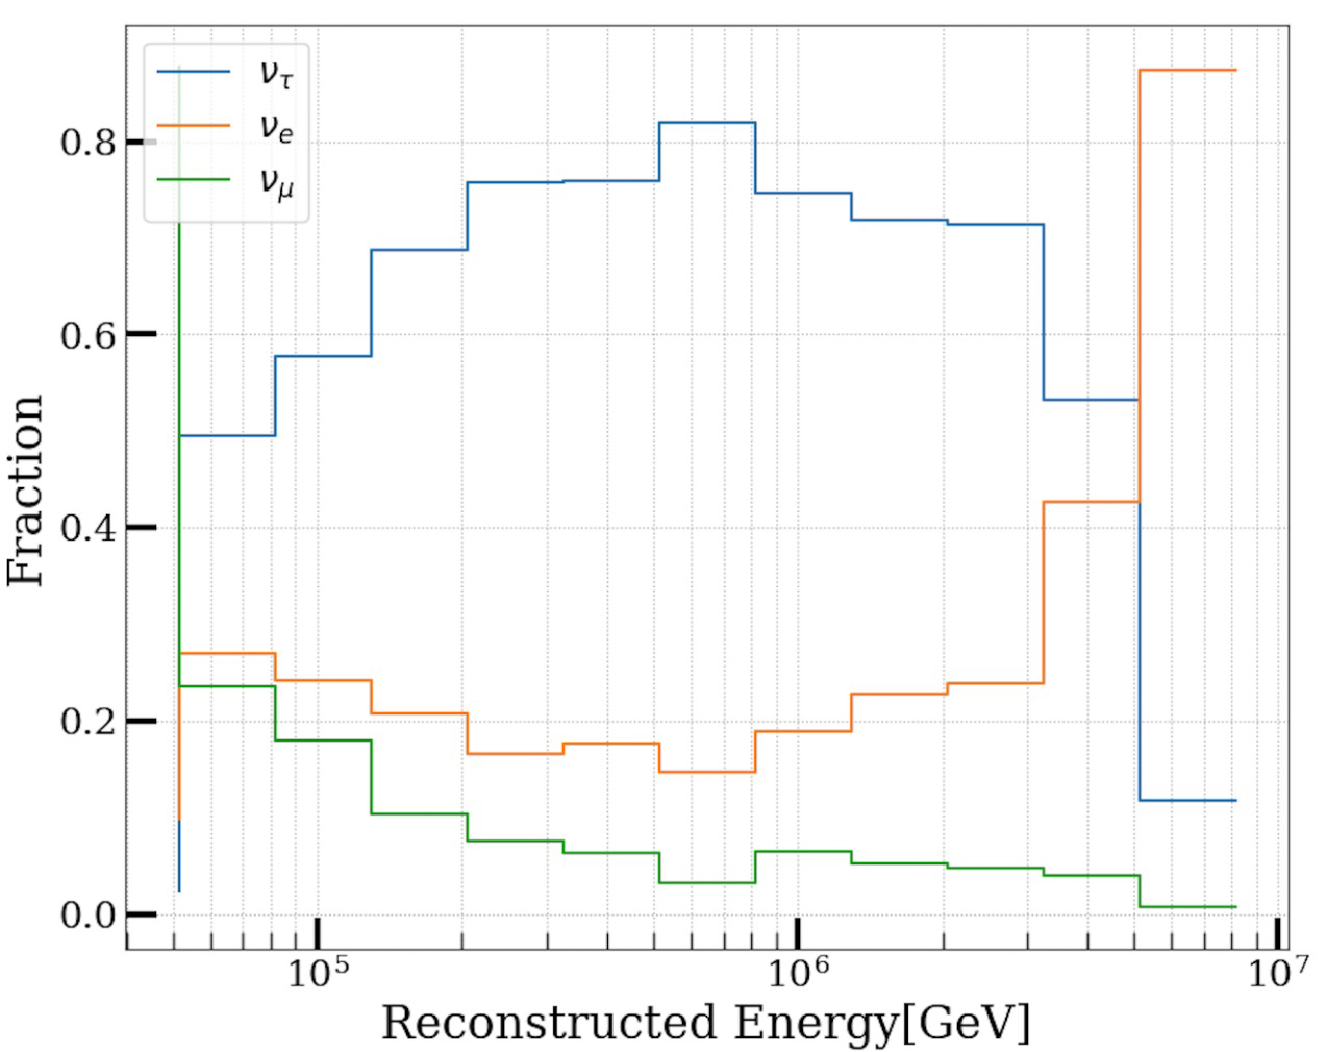
\includegraphics{./figures/EventSample/fraction_nomask.pdf}
    \end{subfigure}
    \hfill
    \begin{subfigure}[h]{0.7\textwidth}
        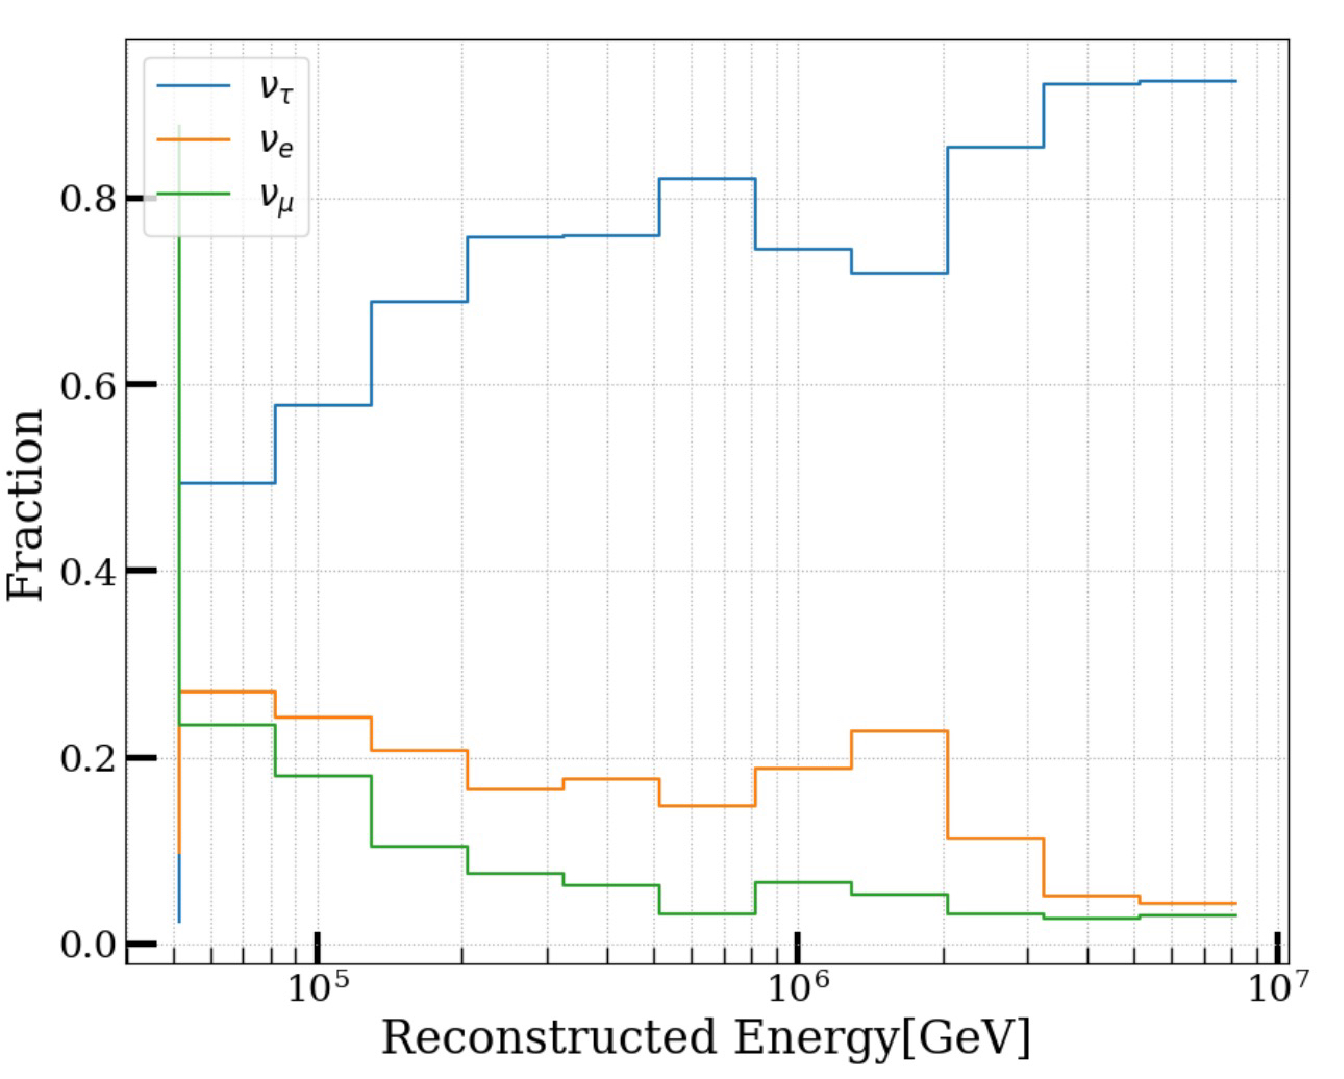
\includegraphics{./figures/EventSample/fraction_withmask.pdf}
       
    \end{subfigure}%
    \caption{Fraction of flavor content per bin in double cascade events. The left panel shows the distribution without the criteria of Total \( E_{\text{deposited}} \geq 3 \) PeV and \( L_{\text{reco}} \leq 20 \) m, indicating \emph{purity contamination} at high energies from \( \bar{\nu}_e \) Glashow events. The right panel presents the distribution after reclassifying double cascades as single cascades under these conditions.}
    \labfig{glashow_mask}
\end{figure*}

To address this, \textbf{a reclassification} mask was introduced at the end of the classification chain outlined in Figure \reffig{PID_chain}. If an event is classified as a Double Cascade with a reconstructed energy of \(\mathrm{E}_{\mathrm{tot}} \geq 3\) PeV and a reconstructed length \(\mathrm{L}_{\mathrm{reco}} \leq 20\) m, it is reclassified as a single cascade. These thresholds were chosen based on the purity distribution to maximize the signal-to-background ratio, even at these energies.The distribution before and after applying this mask is shown in the right panel of Figure \reffig{glashow_mask}. As anticipated, the lower energy distributions remain nearly identical, while purity is restored at higher energies. It is important to note that the fraction of \(\nu_{\mu}\) remains unchanged in both figures, due to the involvement of only electron neutrinos—technically electron anti-neutrinos—in Glashow interactions, which contribute to the purity contamination. Since this is merely a reclassification, the total High-Energy Starting Event (HESE) sample remains unchanged.
 

\subsection{Tau Polarisation}
\label{sec:tau_polarisation}
As discussed in \ref{sec:morphologies}, $\nu_{\tau}$-CC interaction always produces a tau lepton, which has various decay modes. The tau lepton produced in this interaction is polarised, which can siginificantly alter the kinematics of the tau decay \sidecite{Tau_Polarisation, Tau_Polarisation_carlos}. Whether the decay mode is leptonic or hadronic, the fraction of energy going to the decay products ($\frac{E_{hadrons/leptons}}{E_{\tau}}$), is affected if non-zero tau Polarisation is not taken into account. The \texttt{PRPOSAL} software used in simulation presneted in this thesis, to simulate secondary charge particle production, propagation and energy losses does not take into account this factor. That is, the Taus produced in a $\nu_{\tau}-$CC interation is assumed to be produced with no polarisation. Since, the signature which is used for identification of this analysis relies on both, the neutrino interaction cascade and tau decay cascade, not taking in account this correction can lead to an \emph{incomplete} simulation of energy loss profiles. Mainly the energy reconstruction of the second decay cascade, may get affected, which can further alter the Energy asymmetry ($E_{\mathrm{A}}$) of the event, which is used a s aselection variable in Ternary Classifier (see \reffig{PID_chain}). 

\begin{marginfigure}
	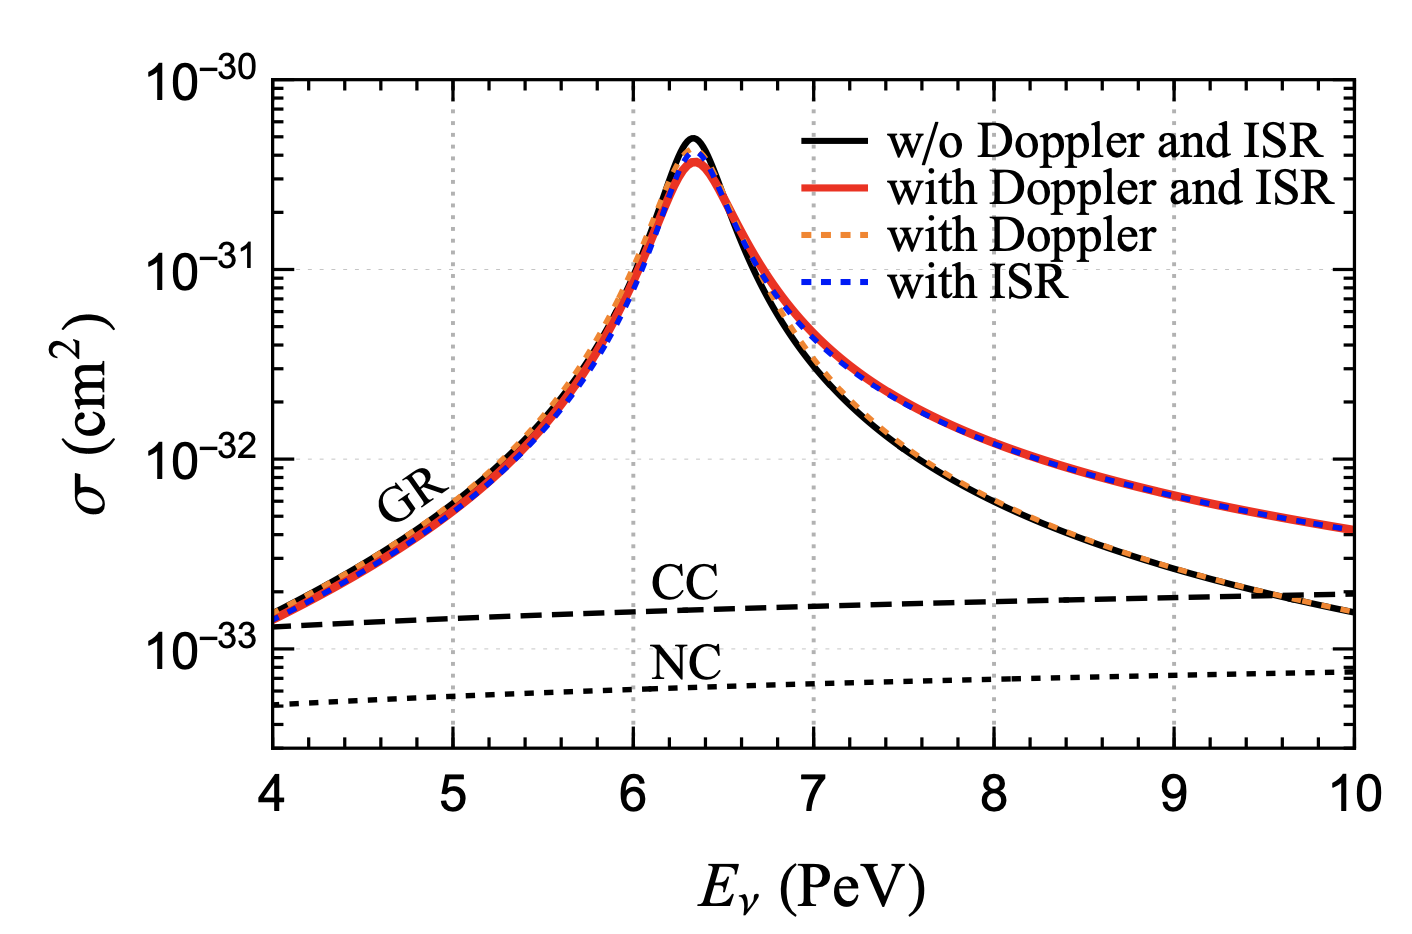
\includegraphics{./figures/EventSample/ISR_glashow.png}
	\caption{The cross section for the Glashow resonance process \(\nu_e +e^- \to W^- \to X\) is shown with and without initial state radiation and Doppler broadening. The black curve represents the cross section without these effects, the blue dotted curve includes initial state radiation, the orange dotted curve shows Doppler broadening, and the red curve combines both effects. Figure taken from \cite{glashow_correcttion1}.}
	\labfig{eff_area}
\end{marginfigure}

The idea is to test the impact of tau polarisation on analysis variables by reweighting the monte carlo events. The calculations provided in \cite{Tau_Polarisation}, are used to get theoretical fractional energy loss of the electromagnetic equivalent visible energy losses, for both polarised and unpolarised states. The ratio of this is multiplied with the simulated fractional energy (which assumed unpolarised taus), to get a new reweighting factor. The change introduced minor difference in the overall observable distributions, hence this was left as a weight correction only and no further analytical checks were performed.


\subsection{Glashow Cross-Section correction}
\label{sec:glashow_correction}
The resonance enhancement of \(\bar{\nu_e}e^-\) scattering at an energy of approximately 6.3 PeV, known as the \emph{Glashow resonance}, was discussed in Section~\ref{sec:glashow}. The cross-section for this process at this energy is significantly larger—about two orders of magnitude greater—than that of Deep Inelastic Scattering (DIS). Since this energy range is relevant to the thesis presented in this work, it is crucial to consider second-order QCD corrections, which can significantly alter the Glashow cross-section \sidecite{glashow_correcttion1}.

The corrections applied to the cross-section, as described in \cite{glashow_correcttion1}, include \emph{Initial State Radiation (ISR)} \sidecite{glashow_correcttion2,glashow_correcttion3} and the \emph{Doppler broadening effect} \sidecite{glashow_correcttion4}. ISR becomes more prominent when the center of mass (COM) energy of the system is much higher than the mass of the initial lepton—since \(W^-\) is substantially more massive than \(e^-\), this leads to an enhancement factor of approximately \(\frac{M_W}{m_e} \sim 12\) in radiation, on top of contributions from the fine structure constant \((\alpha)\). This results in collinear photon emission. Doppler broadening occurs due to the motion of atomic electrons, where the typical velocity of the electron is assumed to be close to the speed of light. This motion causes the COM energy to shift by a factor of \((1 - \beta \cos\theta)\), where \(\theta\) is the angle between the electron's velocity (\(\beta\)) and the incoming neutrino in the lab frame \cite{glashow_correcttion4}. 

The combined results of these effects, based on calculations from \cite{glashow_correcttion1}, were used to adjust the \emph{total weight} of neutrinos. As noted in \cite{glashow_correcttion1}, these effects are smoothed out by the energy resolution of IceCube \sidecite{energy_reco}, and the impact of this reweighting on energy distributions and sensitivity was negligible. Nevertheless, the reweighting was retained, similar to the correction for Tau polarization.

\section{Influence of South Pole Ice properties on Double Cascades Reconstruction}
\label{sec:icemodel_checks}
The identification of $\nu_{\tau}$-induced double cascades in the IceCube detector faces significant systematic uncertainties due to the anisotropy of the ice. As discussed in Section~\ref{sec:icemodel}, the Anisotropy at the south pole ice has been established since 2013 \sidecite{bfr_icrc2013}. This phenomenon causes photons to have a directional dependence while scattering, with enhanced scattering occurring perpendicular to the ice flow axis\sidenote{Technically it coincides within 1\textdegree of the ice flow axis, hence this axis was given a special name, \emph{the anisotropy axis}. The axis along which scattering is reduced is called \emph{the major anisotropy axis} and the one perpendicular to it where scattering is enhanced is known as \emph{the minor anisotropy axis}.} and reduced scattering along it. 

\marginnote{\begin{kaobox}
    While the SpiceBfr model agrees much better with the data, compared to Spice-3.2.1, it is important to note that on the analysis level, where one uses reconstruction algorithms based on all of the pulse information from the DOMs, the ever so significant effects on charge and time level may get smeared off from overall observable distributions. Going from Spice-mie to Spice-Lea was a breakthrough as the former did not consider this anisotropic behavior of photon propagation. But going from Spice-3.2.1 to Spice-Bfr was more in the direction of inherent modeling of the ice (crystal) property, to explain the anisotropy, while Spice-3.2.1 and Spice-Lea used an approximated solution in the form of effectively mimicking an anisotropic scattering of photons.  
\end{kaobox}}

Such a direction dependednt scattering pattern can cause a bias in reconstructing specifically a double cascade event using \texttt{taupede}, as this algorithm looks for energy depositions around vertices along a given seed direction (see Section~\ref{sec:PID}), which can cause bias in length reconstruction. When a single cascade aligns with this major anisotropy axis, reduced scattering can elongate its apparent size, mimicking double cascade characteristics due to altered light timing at the DOMs. Conversely, if a true double cascade aligns with one of the minor anisotropy axes, it may be compressed, increasing the risk of misidentification as a single cascade. Without accounting for anisotropy, true single cascades could be misclassified as double cascades, while genuine double cascades along minor axes might be missed.

Reconstructing these events relies on photo-spline tables introduced in Section~\ref{sec:reco}, which provide tabulated light yields for simulated 1 GeV cascades. These cascades are placed in the detector's center at intervals of $\Delta z = 20$ m, between depths of $-600$ to $600$ m and zenith angles from $0^{\circ}$ to $180^{\circ}$. The initial model primarily considers the ice layer's depth and zenith angle for light propagation, but an additional azimuthal dimension was necessary to account for anisotropy. A key advancement was the development of \textbf{the effective distance spline tables}, which adjusted for anisotropy by using an isotropic-ice-equivalent position instead of position of the DOMs to look-up for the light yield, which resulted in a  significant enhancing of length reconstruction accuracy \sidecite{marcel_thesis}.

Recent developments in icemodel studies have revealed that the directional behavior of light in ice, is due to its molecular structure, a phenomenon known as \emph{birefringence} as already introduced in Section~\ref{sec:icemodel}. This is now incorporated into the new ice model, called as, \textbf{SpiceBfr}. However, during the development stage of the analysis presneted in this thesis, the only large-scale Monte Carlo simulations available was the one produced using an earlier icemodel, \textbf{Spice-3.2.1} \sidenote{This icemodel is almost identical to the one used in previous iteration of this analysis \cite{Juliana_thesis}}. Naturally, the question arises, if SpiceBfr can further improve reconstruction (or discover any previously unknown biases), hence a comparison was needed. 

Such a check between Spice-3.2.1 and SpiceBfr was feasible since the spline tables for SpiceBfr were already available. To facilitate cross-comparison, a small statistics (one-third of the full available statistics) simulation set was produced using SpiceBfr. The succecfully identified true double cascades are considered, and median length bias ($L_{\text{Reco}} - L_{\text{true}}$) is calculated per azimuth bin (see \reffig{lengtbias}). An effective reconstruction algorithm should show no bias (i.e. the difference in length should be zero), unless unaccounted asymmetries exist.
\begin{table*}
    \caption{The four comparison scenarios that were analyzed. The First icemodel in the name always refers to the one used in simulation (second column) and the second refers to the one used in reconstruction (reconstruction). Last column points to corresponding figures.}
    \labtab{anotheruseless}
    \centering
    \begin{tabular}{cccc}
    \hline
    \textbf{Name} & \textbf{Simulation Icemodel} & \textbf{Reconstruction Icemodel} &\\
    \hline
    Spice-3.2.1-Spice-3.2.1 & Spice-3.2.1 & Spice-3.2.1 &\reffig{spicespice} \\
    
    Spice-3.2.1-SpiceBfr & Spice-3.2.1 & SpiceBfr &\reffig{spicebfr} \\
    
    SpiceBfr-Spice-3.2.1 & SpiceBfr & Spice-3.2.1 & \reffig{bfrspice} \\
    
    SpiceBfr-SpiceBfr & SpiceBfr & SpiceBfr & \reffig{bfrbfr} \\
    \hline
    
\end{tabular}
\end{table*}

\begin{figure*}[hbt!]

\begin{subfigure}{.7\textwidth}
    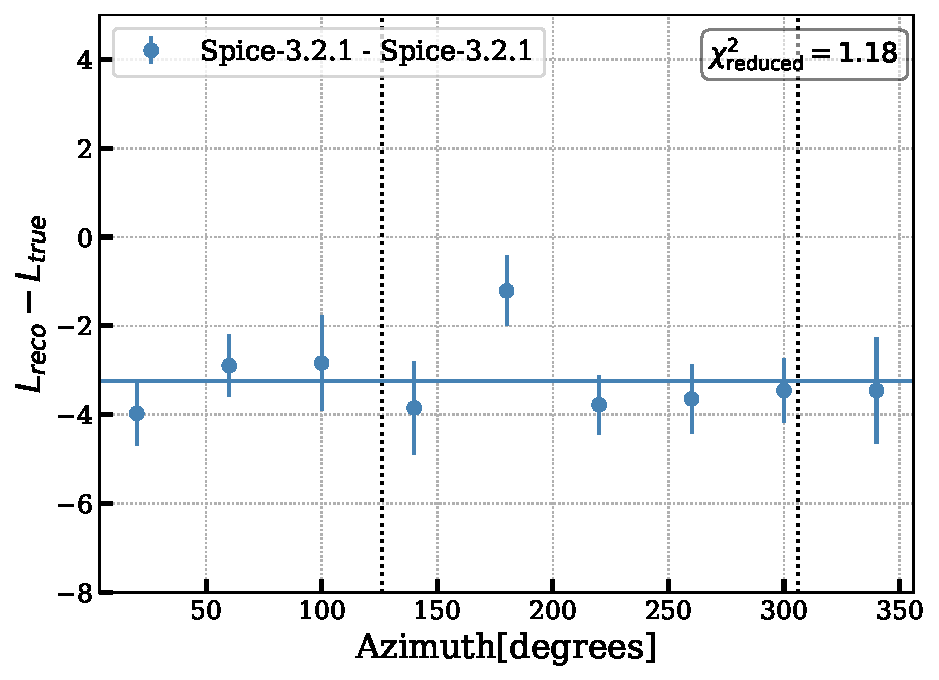
\includegraphics[width=\linewidth]{./figures/EventSample/Lbias_spicespice.pdf}
    \caption{Simulation using Spice-3.2.1 and reconstruction using Spice-3.2.1}
    \labfig{spicespice}
\end{subfigure}\hfill % <-- "\hfill"
\begin{subfigure}{.7\textwidth}
    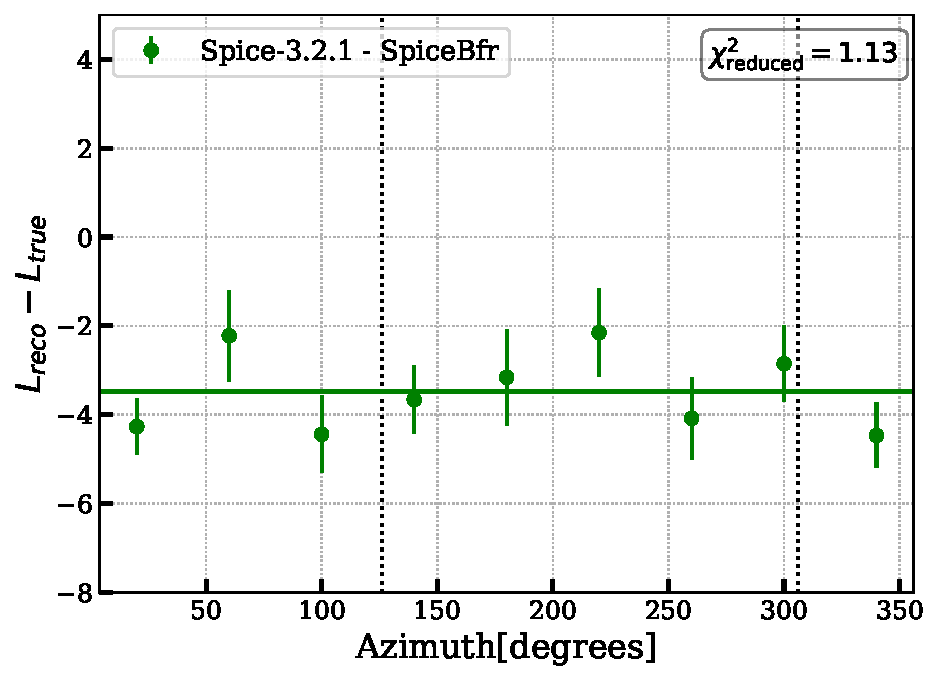
\includegraphics[width=\linewidth]{./figures/EventSample/Lbias_spicebfr.pdf}
    \caption{Simulation using Spice-3.2.1 and reconstruction using SpiceBfr}
    \labfig{spicebfr}
\end{subfigure}

\medskip % create some *vertical* separation between the graphs
\begin{subfigure}{.7\textwidth}
    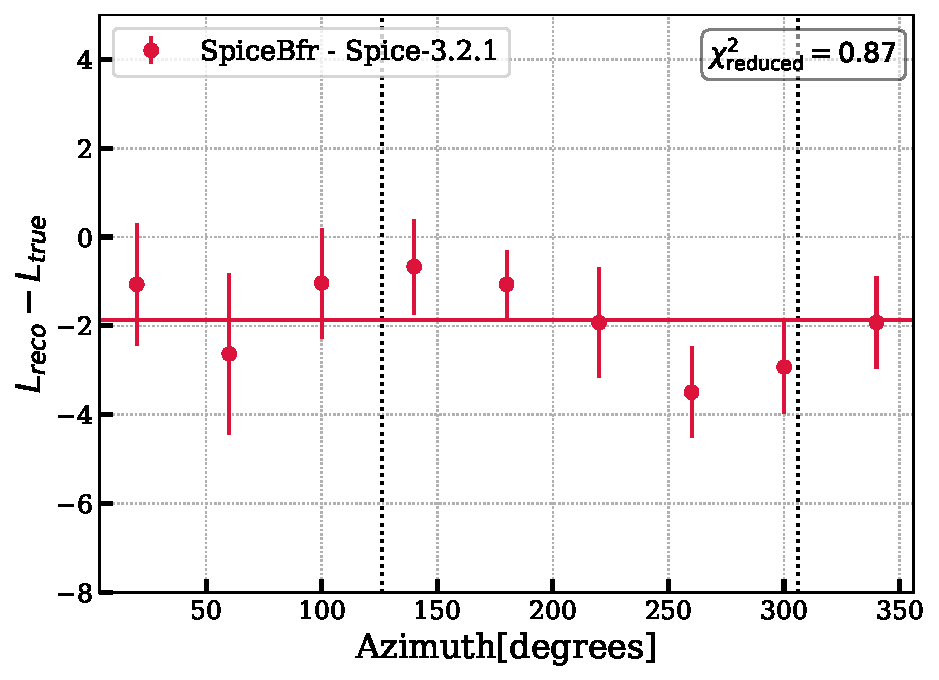
\includegraphics[width=\linewidth]{./figures/EventSample/Lbias_bfrspice.pdf}
    \caption{Simulation using SpiceBfr and reconstruction using Spice-3.2.1}
    \labfig{bfrspice}
\end{subfigure}\hfill % <-- "\hfill"
\begin{subfigure}{.7\textwidth}
    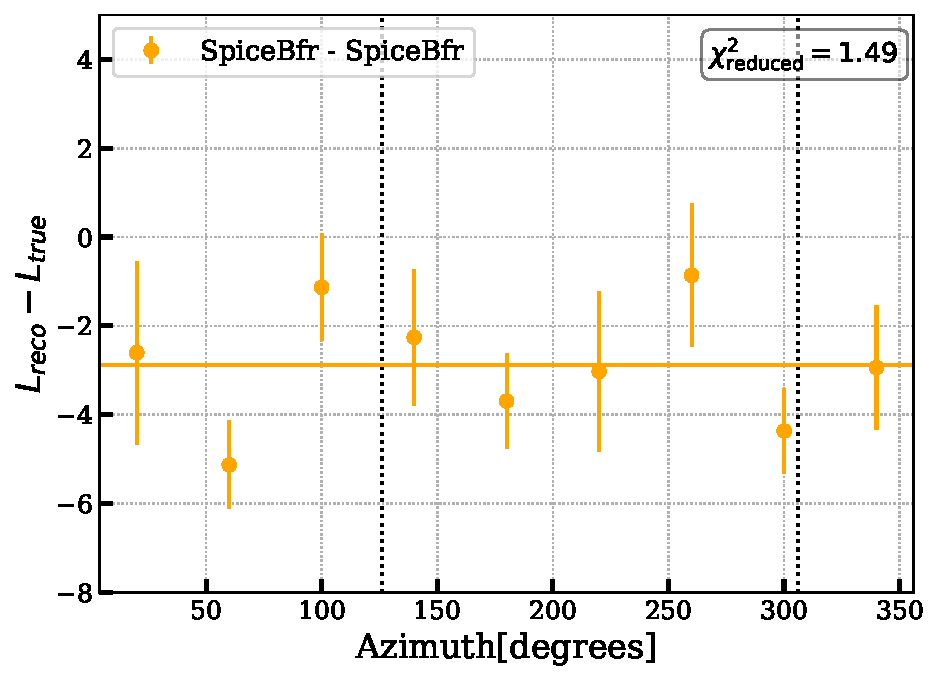
\includegraphics[width=\linewidth]{./figures/EventSample/Lbias_bfrbfr.pdf}
    \caption{Simulation using SpiceBfr and reconstruction using SpiceBfr}
    \labfig{bfrbfr}
\end{subfigure}

\caption{Length Bias of true double cascades, classified as double cascades, as function of Azimuth angle. Vertical lines shows the direction of the major anisotropy axis. Caption below each figures shows which combination of icemodel is used in simulation and reconstruction respectively. Each figure also shows reduced value of $\chi^2$ calculated by fitting the showed horizontal line, see text for details.}
\labfig{lengtbias}
\end{figure*}


Since all cases involve either the effective distance correction or an inherent anisotropy parametrization (via birefringence), minimal bias was expected along the major anisotropy axis. As shown in the results, only minor structures were observed, and none were deemed statistically significant, particularly along the anisotropy axis. To probe further, a $\chi^2$ goodness-of-fit (gof) test was performed to fit a horizontal line, with the reduced $\chi^2$ calculated for each of the four cases (values indicated on all figures). The results indicated that all four combinations fit well to a horizontal line, signifying no significant biases were present. However, the plots corresponding to the simulation produced using SpiceBfr (both reconstructed with SpiceBfr (\reffig{bfrbfr}) and Spice-3.2.1 \reffig{bfrspice}) showed signs of over/underfitting, likely due to the low statistics of the generated SpiceBfr simulation set. 

\begin{marginfigure}
    
    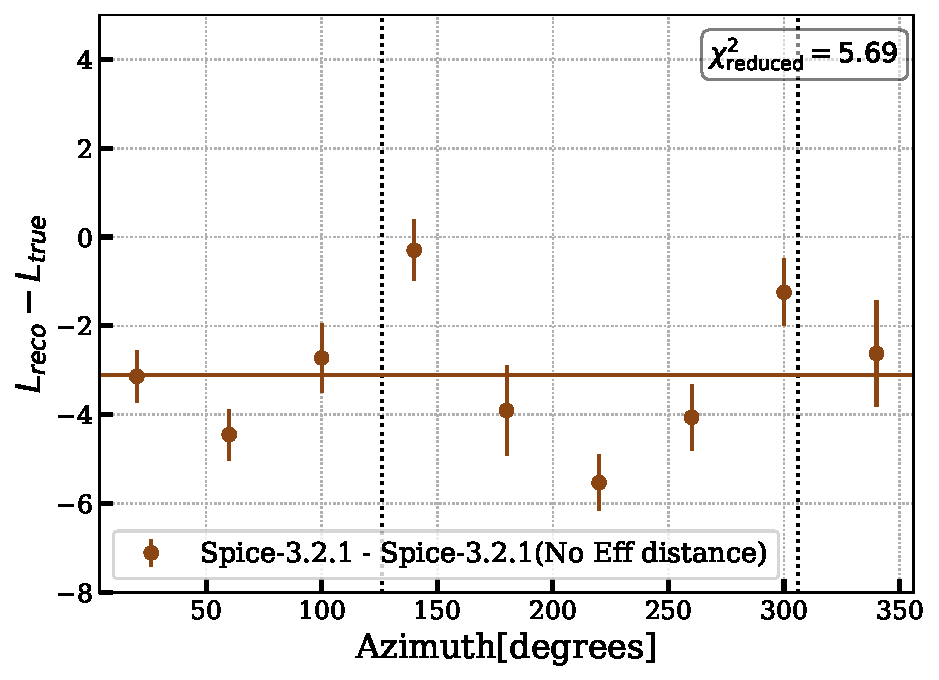
\includegraphics{./figures/EventSample/Lbias_spicenoeffdist.pdf}
    \caption{Simulation using Spice-3.2.1 and reconstruction using Spice-3.2.1 but no effective distance. See caption of \reffig{lengtbias} for details.}
    \labfig{noeff_dist}
\end{marginfigure}

This observed lack of obias aligns with expectations, as Spice-3.2.1 effectively handles anisotropy through the effective distance parameterization. The final step thus, was to verifying if the lack of bias was truly due to the effective distance splines. In \reffig{noeff_dist}, a distribution is shown where events are simulated using Spice-3.2.1 but reconstructed without the effective distance correction. The resulting reduced $\chi^2$ of 5.69 indicates a poor fit, and a clear bias is visible along the anisotropy axis, as was observed in \cite{marcel_thesis}. This conclusively demonstrates that both Spice-3.2.1 and SpiceBfr, both with appropriate effetive distance corrections are well-suited for analyzing $\nu_{\tau}$-induced double cascades in the presence of ice anisotropy.

Since the SpiceBfr model represents the best current understanding of South Pole ice, the decision was made to proceed with simulations using Spice-3.2.1, reconstructed with the SpiceBfr model. This choice is further supported by the reduced $\chi^2$ values across the four cases, where the combination of Spice-3.2.1 simulation and SpiceBfr reconstruction produced the value closest to 1, indicating the most accurate fit. Consequently, the analysis continued with this combination, ensuring the best possible handling of ice anisotropy in the event reconstruction.

Given that the SpiceBfr model represents the best current understanding of the South Pole ice, the decision was made \textbf{to proceed with Spice-3.2.1 simulations reconstructed using the SpiceBfr model}. This approach is further supported by the reduced $\chi^2$ values across the four cases, with the Spice-3.2.1 simulation and SpiceBfr reconstruction yielding the value closest to 1, indicating the most accurate fit. Hence, from here-on, it is to be 





    

